\documentclass[12pt]{report}
\usepackage[a4paper, portrait, margin=1cm, bottom=2cm]{geometry}
\usepackage{fontspec}
\usepackage[fleqn]{amsmath}
\usepackage{amssymb}
\usepackage{graphicx}
\usepackage{indentfirst}
\usepackage{polyglossia}
\usepackage[dvipsnames]{xcolor}
\usepackage{physics}

\setmainfont[Ligatures=TeX]{Linux Libertine}
\setmainlanguage{russian}
\setotherlanguages{english}
\graphicspath{graphics}

\begin{document}

\chapter{Вопросы по теории}

\section{Система уравнений Максвелла, физический смысл уравнений.}
Система уравнений Максвелла — система уравнений в дифференциальной или интегральной форме, описывающих электромагнитное поле и его связь с электрическими зарядами и токами в вакууме и сплошных средах. Физический смысл --- описание электромагнитного поля.

\begin{tabular}{|l|l|l|}
    \hline
                                         & Дифференциальная форма                                        & Интегральная форма                                                                            \\
    \hline
    Закон Гаусса                         & $\displaystyle \nabla \cdot \vec D = \rho$                    & $\displaystyle \oint_S \vec D \cdot \dd s = Q$                                                \\
    \hline
    Закон Гаусса для магнитного поля     & $\nabla \cdot \vec B = 0$                                     & $\displaystyle \oint_S \vec B \cdot \dd s = 0$                                                \\
    \hline
    Закон индукции Фарадея               & $\nabla \times \vec E = -\dfrac{\dd{\vec B}}{\dd{t}}$         & $\displaystyle \oint_l \vec E \cdot \dd l = -\dfrac{\dd}{\dd{t}}\int_S \vec B \cdot \dd S$    \\
    \hline
    Теорема о циркуляции магнитного поля & $\nabla \times \vec H = \vec j + \dfrac{\dd{\vec D}}{\dd{t}}$ & $\displaystyle \oint_l \vec H \cdot \dd l = I + \dfrac{\dd}{\dd t} \int_S \vec D \cdot \dd S$ \\
    \hline
\end{tabular}

Где:
\begin{itemize}
    \item $\rho$ --- объёмная плотность (стороннего) электрического заряда ($\dfrac{\text{Кл}}{\text{м}^3}$).
    \item $\vec j$ --- плотность электрического тока ($\dfrac{\text{А}}{\text{м}^2}$).
    \item $\vec E$ --- напряженность электрического поля ($\dfrac{\text{В}}{\text{м}}$).
    \item $\vec H$ --- напряжённость магнитного поля ($\dfrac{\text{А}}{\text{м}}$).
    \item $\vec D$ --- электрическая индукция ($\dfrac{\text{Кл}}{\text{м}^2}$).
    \item $\vec B$ --- магнитная индукция ($\text{Тл} = \dfrac{\text{Вб}}{\text{м}^2} = \dfrac{\text{кг}}{\text{с}^2\text{А}}$).
    \item $\nabla$ --- дифференциальный оператор набла, при этом:
          \begin{itemize}
              \item $\nabla \times \vec E \equiv \text{rot} E$ означает ротор вектора $E$
              \item $\nabla \cdot \vec E \equiv \text{div} E$ означает дивергенцию вектора $E$
          \end{itemize}
    \item $Q$ --- суммарный электрический заряд
    \item $I$ --- электрический ток
\end{itemize}

\subsection{Материальные уравнения, дополняющие систему уравнений Максвелла}
\begin{align*}
     & \vec D = \varepsilon \varepsilon_0 \vec E \\
     & \vec B = \mu \mu_0 \vec H                 \\
     & \vec j = \gamma \vec E                    \\
\end{align*}
Где:
\begin{itemize}
    \item $\varepsilon_0 = 8.85 \cdot 10^{-12} \dfrac{\text{Ф}}{\text{м}}$ --- электрическая постоянная
    \item $\varepsilon$ --- диэлектрическая проводимость среды
    \item $\mu_0 = 1.25 \cdot 10^{-6} \dfrac{\text{Гн}}{\text{м}}$ --- магнитная постоянная
    \item $\mu$ --- магнитная проницаемость среды
    \item $\gamma$ --- удельная проводимость
\end{itemize}

\section{Закон сохранения электрического заряда. Закон Кулона. Напряженность электрического поля и потенциал, и связь между ними. Интегральная и дифференциальная форма уравнений электростатического поля в вакууме. Электрическое поле при наличии вещества (проводников и диэлектриков).}
\subsection{Закон сохранения электрического заряда}
Алгебраическая сумма зарядов электрически замкнутой системы сохраняется:
\[
    q_1 + q_2 + q_3 + \dots + q_n = const
\]

\subsection{Закон Кулона}
Физический закон, описывающий взаимодействие между двумя неподвижными точечными зарядами в вакууме. Сила, с которой заряд $q_1$ действует на заряд $q_2$, согласно этому закону, находится, как:
\[
    \vec F_{12} = \dfrac{q_1 q_2 \vec r}{4\pi \varepsilon \varepsilon_0 \abs{\vec r}^3}
\]
Где $\vec r$ --- вектор, построенный от заряда $q_1$ к заряду $q_2$, $\varepsilon_0 \approx 8.85 \cdot 10^{-12} \dfrac{\text{Ф}}{\text{м}}$ --- электрическая постоянная, $\varepsilon$ --- диэлектрическая проницаемость среды

\subsection{Напряженность электрического поля и потенциал, и связь между ними}
\subsubsection{В электростатике:}
Напряженность электрического поля --- векторная физическая величина, характеризующая электрическое поле в данной точке и равная отношению силы $\vec F$, действующей на неподвижный малый по величине точечный заряд, помещённый в данную точку, к величине этого заряда $q^*$:
\[
    \vec E = \dfrac{\vec F}{q^*} \ \dfrac{\text{А}}{\text{м}}
\]

Через закон Кулона можно записать напряжённость так ($q$ --- точечный заряд, образующий поле, $r$ --- вектор от $q$ до точки измерения):
\[
    \vec E = \dfrac{q \cdot \vec{r}}{4\pi \varepsilon_0 \varepsilon \abs{\vec{r}}^3}
\]

Потенциал --- скалярная характеристика электростатического поля, характеризующая потенциальную энергию, которой обладает единичный положительный заряд, помещённый в данную точку поля. Он равен отношению потенциальной энергии взаимодействия заряда с полем к величине этого заряда:
\[
    \phi = \dfrac{W_p}{q_0} \ \text{В}
\]
Где:
\begin{itemize}
    \item $W_p = \dfrac{q_0q}{4\pi\varepsilon_0\varepsilon r}$ --- потенциальная энергия заряда $q_0$ в поле заряда $q$ на расстоянии $r$ от него.
\end{itemize}

Связь потенциала и напряжённости:
\[
    \vec E = - \grad \phi \\ \phi = - \int \vec E \cdot \vec \dd{r} \\ \phi = \abs{\vec{E}} \cdot r
\]
\subsection{Интегральная и дифференциальная форма уравнений электростатического поля в вакууме}
\begin{tabular}{|l|l|l|}
    \hline
                                         & Дифференциальная форма                                        & Интегральная форма                                                                            \\
    \hline
    Закон Гаусса                         & $\displaystyle \nabla \cdot \vec D = \rho$                    & $\displaystyle \oint_S \vec D \cdot \dd s = Q$                                                \\
    \hline
    Закон Гаусса для магнитного поля     & $\nabla \cdot \vec B = 0$                                     & $\displaystyle \oint_S \vec B \cdot \dd s = 0$                                                \\
    \hline
    Закон индукции Фарадея               & $\nabla \times \vec E = -\dfrac{\dd{\vec B}}{\dd{t}}$         & $\displaystyle \oint_l \vec E \cdot \dd l = -\dfrac{\dd}{\dd{t}}\int_S \vec B \cdot \dd S$    \\
    \hline
    Теорема о циркуляции магнитного поля & $\nabla \times \vec H = \vec j + \dfrac{\dd{\vec D}}{\dd{t}}$ & $\displaystyle \oint_l \vec H \cdot \dd l = I + \dfrac{\dd}{\dd t} \int_S \vec D \cdot \dd S$ \\
    \hline
\end{tabular}

\subsection{Электрическое поле при наличии вещества (проводников и диэлектриков)}
\begin{align*}
     & \vec D = \varepsilon \varepsilon_0 \vec E \\
     & \vec j = \gamma \vec E                    \\
\end{align*}

\section{Сила Лоренца. Сила Ампера. Закон электромагнитной индукции Фарадея.}
\subsection{Сила Лоренца}
\textbf{Опр.} Сила, действующая на заряженную частицу со стороны магнитного и электрического поля, называется \textrm{\underline{\textit{силой Лоренца:}}}
\[
    \vec{F_\textrm{Л}} = q\vec{E} + q\vec{\upsilon}\times\vec{B}
\]
Часто под силой Лоренца подразумевается лишь магнитная её составляющая $F_\textrm{Л} \approx q\vec{\upsilon}\times\vec{B}$

\subsection{Сила Ампера}
Сила ампера --- сила, с которой магнитное поле, характеризуемое вектором магнитной индукции $\vec B$, действует на элементарный отрезок проводника $\dd l$, по которому течёт ток $I$:
\[
    \dd{\vec F_A} = I \dd{\vec{l}} \times \vec{B}
\]

\subsection{Закон электромагнитной индукции Фарадея}
ЭДС электромагнитной индукции в контуре численно равна и противоположна по знаку скорости изменения магнитного потока сквозь поверхность, натянутую на этот контур. ЭДС возникает, если поток $\Phi_B$ изменяется по любым причинам.
\[
    \varepsilon_i = - \dfrac{\dd{\Phi_B}}{\dd t}
\]

\section{Волновое уравнение для электромагнитной волны в вакууме. Плоская монохроматическая волна.}
Волновое уравнение для электромагнитной волны в вакууме:
\[
    \Delta \vec{E} - \dfrac{1}{c^2} \dfrac{\dd^2}{\dd{t^2}} = 0 \qquad \Leftrightarrow \qquad \square \vec E = 0
\]

Плоские монохроматические волны --- это волны одной строго определённой частоты. Они являются решениями волнового уравнения элекромагнитного поля.
\[
    \vec E(\vec r, t) = \widetilde{E}_0\cos(\omega t - \vec{k}\cdot \vec{r} + \phi_0)\vec{e}_p
\]
Где
\begin{itemize}
    \item $\widetilde{E}_0$ --- вещественная амплитуда плоской волны
    \item $\vec{k}$ --- волновой вектор
    \item $\omega$ --- циклическая частота монохроматической волны
    \item $\phi_0$ --- начальная фаза волны
    \item $\vec{e}_p$ --- единичный вектор поляризации световой волны
    \item $\omega t - \vec{k} \cdot \vec{r} + \phi_0$ --- фаза волны
\end{itemize}

\section{Принцип Гюйгенса-Френеля. Дифракция света на круглом отверстии.}
\subsection{Принцип Гюйгенса-Френеля}
\subsubsection{Принцип Гюйгенса}
Каждый элемент поверхности, которой достигла в данный момент волна, является центром элементарных волн, огибающая которых будет волновой поверхностью в следующий момент времени.

Этот принцип позволяет найти положение фронта волны в момент времени $t + \Delta t$, зная его положение в предыдущий момент времени $t$ и скорость волны $v$.

\subsubsection{Дополнение Френеля принципу Гюйгенса}
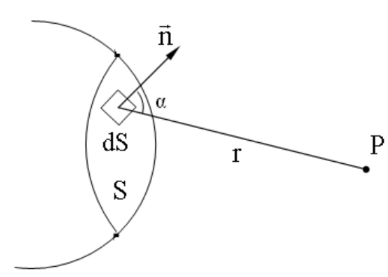
\includegraphics{graphics/05_1.png}
\begin{enumerate}
    \item Вторичные источники не точечные, а элементы фронта волны площадью $dS$
    \item Вторичные источники $\dd S$ --- когерентные и результат их действия на точку $P$ есть результат интерференции
    \item Площадка фронта волны $\dd S$ создаёт в точке $P$ напряжённость ЭП:
          \[
              \dd{E} \sim \dd{S} \\ \dd{E} \sim A_0 \\ \dd{E} \sim \alpha \\ \dd{E} \sim \dfrac{I}{r}
          \]
          Где:
          \begin{itemize}
              \item $A_0$ --- амплитуда световой волны в месте, где находится Площадка
              \item $\alpha$ --- угол между нормалью к площадке $\dd{S}$ и направлением на точку $P$
              \item $r$ --- расстояник от площадки $\dd S$ до точки $P$
          \end{itemize}
\end{enumerate}

Принцип Гюйгенса-Френеля позволяет объяснить дифракцию КОЛИЧЕСТВЕННО и решить любую задачу на дифракцию света.

\subsection{Дифракция света на круглом отверстии}
\begin{center}
    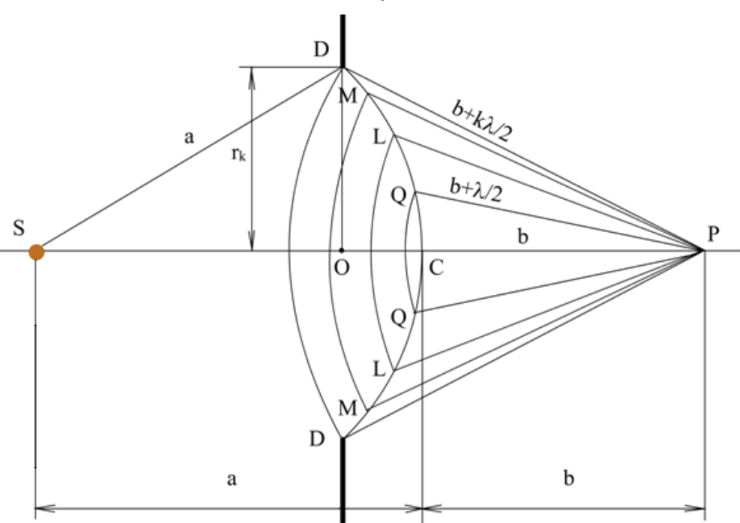
\includegraphics[width=0.5\textwidth]{graphics/05_2.png}
\end{center}
Разобьем открытую часть волновой поверхности на зоны Френеля:
\[
    r_m = \sqrt{\dfrac{ab}{a + b}m\lambda}
\]

Колебания от двух соседних зон (например, $Q$ и $L$) приходят в противофазе.

\section{Дифракция Фраунгофера. Дифракционная решетка.}

\subsection{Дифракция Фраунгофера}
Рассмотрим падение плоской монохроматической световой волны на длинную узкую прямую щель, вырезанную в непрозрачном для света экране.

Свет проходит сквозь щель и линзу, помещённую параллельно непрозрачному экрану.  Дифракционную картину наблюдают на экране, расположенном в фокальной плоскости линзы.

Из всей совокупности вторичных когерентных волн плоского фронта волны, расположенного в щели, выделим лучи, идущие под углом $\phi$ к главной
оптической оси линзы.

\begin{center}
    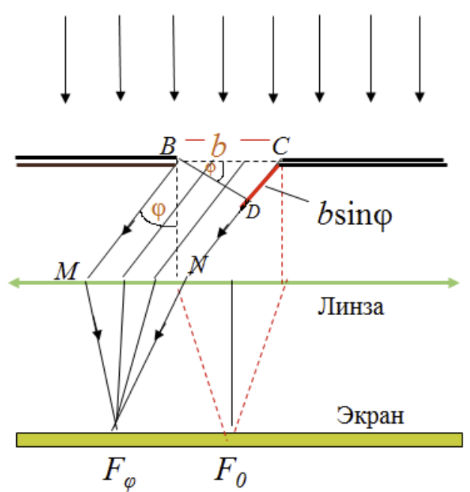
\includegraphics[width=0.5\textwidth]{graphics/06_2.png}
\end{center}

\begin{itemize}
    \item $b$ --- ширина щели
    \item $\phi$ --- угол дифракции
    \item $\lambda$ --- длина волны света
    \item $k$ --- порядок максимума
\end{itemize}

Зоны Френеля выглядят как полоски, параллельные щели. Ширина зоны Френеля:
\[
    x = \dfrac{\lambda / 2}{\sin \phi}
\]

Количество зон Френеля, уложившихся на ширине щели:
\[
    N = \dfrac{b}{x} \\ N = \dfrac{b\sin \phi}{\lambda / 2}
\]

В точке $P$ экрана будут наблюдаться:
\begin{itemize}
    \item максимумы, если в эту точку свет приходит от нечётного числа зон Френеля: $N = 2k + 1$
    \item минимумы, если свет приходит от чётного числа зон Френеля: $N = 2k$
\end{itemize}

\subsection{Дифракционная решётка}
Дифракционная решётка — оптический прибор, представляющий собой периодическую структуру из большого числа регулярно расположенных элементов, на которых происходит дифракция света (например, параллельных и равноотстоящих штрихов, нанесённых на плоскую или вогнутую оптическую поверхность).

\begin{center}
    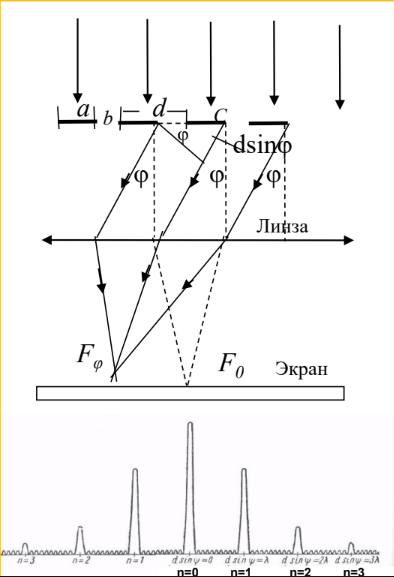
\includegraphics[width=0.5\textwidth]{graphics/06_1.png}
\end{center}

Штрихи с определённым и постоянным для данной дифракционной решётки профилем повторяются через одинаковый промежуток $d$, называются её периодомЖ
\[
    d = a + b
\]

Если решётка имеет $N$ щелей на длине $L$, то:
\[
    d = \dfrac{L}{N}
\]

\section{Расчет интерференционной картины в опыте Юнга на основе волновой теории.}
В опыте Юнга свет от источника, в качестве которого служила узкая щель $S$, падал на экран с двумя близко расположенными щелями $S_1$ и $S_2$. На экране Э световые пучки, прошедшие через щели $S_1$ и $S_2$, перекрывались.  В области перекрытия световых пучков наблюдалась интерференционная картина в виде чередующихся светлых и темных полос.

\begin{center}
    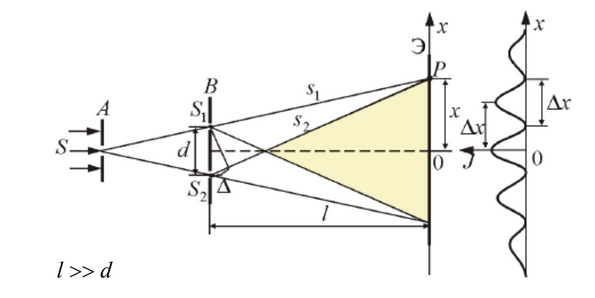
\includegraphics[width=100mm]{graphics/07.png}
\end{center}
\begin{center}
    $S^2 _2 = l^2 + (x + \frac{d}{2})^2 $
\end{center}
\begin{center}
    $S^2 _1 = l^2 + (x + \frac{d}{2})^2 $
\end{center}
\begin{center}
    $S^2 _2 - S^2 _1 = (S_2 + S_1)(S_2 - S_1) = 2xd $
\end{center}
\begin{center}
    $\Delta = S^2 _2 - S^2 _1 = \frac{2xd}{S_1 + S_2}$
\end{center}
\begin{center}
    $\Delta = (S_1 + S_2) ≈ 2l$
\end{center}
\begin{center}
    $l >> d$
\end{center}
\begin{center}
    $\Delta = \frac{xd}{l}$
\end{center}
\begin{center}
    $\Delta = \frac{xd}{l}$ - оптическая разность хода
\end{center}
\begin{center}
    $x_max = \pm m \frac{l}{d} \lambda_0, (m = 0, 1, 2, ...) $ - максимумы интенсивности
\end{center}

Ширина интерференционной полосы – расстояние между двумя соседними интерференционными максимумами (или минимумами):

\begin{center}
    $\Delta x = \frac{l}{d} \lambda_0$, где  $\lambda_0$ - длина волны в вакууме
\end{center}

Ширина интерференционной полосы не зависит от порядка интерференции (величины $m$) и является постоянной для заданных $l$, $d$ и $\lambda_0$

\section{Закон сохранения электрических зарядов. Закон Кулона.}
\subsection{Закон сохранения электрических зарядов.}
Закон сохранения электрических зарядов - Суммарный заряд электрически
изолированной системы сохраняется.
\subsection{Закон кулона}
\subsubsection{В скалярной форме:}
Сила электростатического взаимодействия F
двух точечных неподвижных зарядов,
находящихся в вакууме, прямо
пропорциональна произведению этих
зарядов $q_1$ и $q_2$, обратно пропорциональна
квадрату расстояния r между зарядами и
направлена вдоль соединяющей их прямой.
\begin{center}
    $F = k \frac{|q_1 q_2|}{r^2}$
\end{center}
\begin{center}
    $k = \frac{1}{4 \pi \varE_0}$
\end{center}
\begin{center}
    $\varE_0 = 8.85 * 10^{-12}$
\end{center}
\subsubsection{В векторной форме}
\begin{center}
    $\vec{F _{12}} = k \frac{q_1 q_2}{r^2}\frac{\overrightarrow{r_{12}}}{r}$
\end{center}
$\vec{F _{12}}$ -  сила, действующая на заряд $q_1$ со стороны заряда $q_2$\\
$\overrightarrow{r _{12}}$ -  радиус-вектор, соединяющий заряд $q_1$ с зарядом $q_2$
\section{Электрическое поле. Напряженность электрического поля.
  Принцип суперпозиции. Изображение электрического
  поля с помощью силовых линий. Поле диполя.}
\subsection{Электрическое поле}
Электрическое поле — вид материи, который окружает каждый электрический заряд, а также возникает при наличии изменяющегося во времени магнитного поля, и оказывает силовое воздействие на все покоящиеся заряды, притягивая или отталкивая их.

\subsection{Напряженность электрического поля}
Напряженность электрического поля - отношение силы $\vec{F}$, действующей со стороны поля на неподвижный точечный пробный электрический заряд, помещенный в рассматриваемую точку поля, к этому заряду.

\begin{center}
    $E = \frac{\vec{F}}{q}$
\end{center}

Пробный электрический заряд должен быть столь малым, чтобы его внесение в поле не вызывало изменения значений и перераспределения в пространстве электрических зарядов, напряженность поля которых измеряется с его помощью.

\subsection{Принцип суперпозиции}
Напряженность электрического поля системы точечных зарядов равна сумме напряженностей полей каждого из этих зарядов в отдельности.
\begin{center}
    $\vec{E} = \displaystyle\sum_{i}\vec{E}_i$
\end{center}
\subsection{Изображение электрического
    поля с помощью силовых линий.}
Силовые линии - линии, проведенные в поле так, что касательные к ним в
каждой точке совпадают по направлению с вектором
напряженности поля.\\
\begin{enumerate}
    \item Линия напряженности считается направленной так же, как вектор $\vec{E}$ поля в рассматриваемой точке линии.
    \item Линии напряженности не пересекаются.
    \item Силовые линии начинаются и заканчиваются только на зарядах, или уходят и приходят в бесконечность.
    \item Число силовых линий на единицу поверхности площадки, перпендикулярной линиям, пропорционально величине $E$ в районе этой площадки $(E_A > E_B)$.
\end{enumerate}

\subsection{Поле диполя}
Электрический диполь – система, состоящая из двух одинаковых по величине, но разноименных точечных зарядов ($\pm q$), расстояние $l$ между которыми мало по сравнению с расстоянием $r$ от этой системы до рассматриваемых точек ее поля.

Плечом диполя - $\vec{l}$ называется вектор, направленный по оси диполя от отрицатель-ного заряда к положительному, модуль которого равен расстоянию между ними.

Электрическим моментом диполя, или дипольным моментом - $\vec{p}$ называется вектор, совпадающий по направлению с плечом диполя и равный произведению модуля заряда½Q½на плечо $\vec{l}$:
\section{Поток вектора напряженности электрического поля.
  Теорема Гаусса, ее применение к расчету электростатических полей.}
\subsection{Поток вектора напряженности электрического поля.}
Потоком вектора напряженности Ф электрического поля через площадку S называется скалярная физическая величина,
равная произведению площади S на нормальную составляющую напряжённости электрического поля E. , где n — вектор нормали к поверхности S, α — угол между нормалью n и вектором напряжённости E.
\subsection{Теорема Гаусса, ее применение к расчету электростатических полей.}
Теорема Гаусса: Поток вектора напряженности электростатического поля черерз произвольную замкнутую поверхность равен сумме всех зарядов, заключенных в этой поверхности, деленому на электрическую постоянную.
\begin{center}
    $\oint \vec{E}\differential\vec{S} = \frac{q}{\varE_0}$
\end{center}
Чтобы найти поле E внутри заряженного цилиндра рассмотрим
применение теоремы Гаусса к соосному цилиндру с радиусом r ≤ R и длиной $l$.
$\rho$ - объемная плотность заряда.
\begin{center}
    $E = 2 \pi \rho r$, при $r ≤ R$
\end{center}
Найдем теперь поле $\vec{E}$ снаружи заряженного цилиндра при r ≥ R.
Рассмотрим цилиндр с радиусом r ≥ R и высотой $l$.
\begin{center}
    $E = \frac{2 \rho \pi R^2}{r}$, при r ≥ R.
\end{center}
\par Здесь объем $V = \pi R^2 l$, так как только в этой части объема $\pi r^2 l$ есть
заряды.
\par Для цилиндра по плоскости

\begin{center}
    $E   = \frac{4 \pi \sigma  R(R + l)}{r(r + l)}$, при r <= R:
\end{center}
\par Для плоскости
\begin{center}
    $E = \frac{\sigma}{2 \varE_0} $
\end{center}
\par  Для сферы
\begin{center}
    $E = k \frac{q}{r^2}$ при r > R, E = 0 при r < R,
\end{center}
\par Для шара
\begin{center}
    $E = k \frac{q}{r^2}$, при r > R, $E = k \frac{Q}{R^3}r$, при r < R
\end{center}
\section{Работа по перемещению заряда в электростатическом поле. Потенциальный характер электростатического поля. Потенциал точечного заряда. Связь между напряженностью электростатического поля и потенциалом.}
\subsection{Работа по перемещению заряда в электростатическом поле.}
Работа сил электростатического поля
при перемещении заряда q из точки 1 в
точку 2 равна произведению перемещаемого заряда на разность
потенциалов в начальной и конечной точках.
\begin{center}
    $A_{12} = q (\varphi_1 - \varphi_2)$
\end{center}
\subsection{Потенциальный характер электростатического поля}
Потенциальный характер электростатического поля - Физическая величина, определяемая
отношением потенциальной энергией
взаимодействия заряда с полем к величине
этого заряда.\\
Потенциальная энергия заряда $q_0$ в поле
заряда $q$ на расстоянии r от него:
\begin{center}
    $W_p = \frac{q_0 q}{4 \pi \varE_0 r}$
\end{center}
\par Потенциал электростатического поля:
\begin{center}
    $\varphi =  \frac{W_p}{q_0}$
\end{center}
\subsection{Потенциал
    точечного заряда}
\begin{center}
    $\varphi =  \frac{q}{4 \phi \varE_0 r}$, где \\
    r – расстояние от данной точки до заряда q, создающего поле.
\end{center}
\subsection{Связь между напряженностью электростатического
    поля и потенциалом}
Напряженность как градиент Потенциала
\begin{center}
    $\varphi_1 - \varphi_2 = \int \vec{E} \differential \vec{l}$
\end{center}
\par Представив это соотношение в дифференциальной форме, получим:
\begin{center}
    $\vec{E} \differential \vec{l} = - \differential \varphi$
\end{center}
\begin{center}
    $\vec{E} \differential \vec{l} = E_l \differential l$, тогда
\end{center}
\begin{center}
    $E_l  = -\frac{\partial \varphi}{\partial l}$
\end{center}
\begin{center}
    $\vec{E} \differential \vec{l}  = E_x \differential x$
\end{center}
\begin{center}
    $\vec{E}  = \vec{E_x} \vec{e}_x +  \vec{E_y} \vec{e}_y +  \vec{E_z} \vec{e}_z$
\end{center}
\begin{center}
    $\vec{E_x} = -\frac{\partial \varphi}{\partial x}$, $\vec{E_y} = -\frac{\partial \varphi}{\partial y}$, $\vec{E_z} = -\frac{\partial \varphi}{\partial z}$
\end{center}
\begin{center}
    $\vec{E} = \vec{E}_x + \vec{E}_y + \vec{E}_z = -(\frac{\partial \varphi}{\partial x} \vec{e}_x +  \frac{\partial \varphi}{\partial y} \vec{e}_y +  \frac{\partial \varphi}{\partial z} \vec{e}_z)$
\end{center}
\begin{center}
    $\grad \varphi = (\frac{\partial \varphi}{\partial x} \vec{e}_x +  \frac{\partial \varphi}{\partial y} \vec{e}_y +  \frac{\partial \varphi}{\partial z} \vec{e}_z) = grad \varphi$
\end{center}
\begin{center}
    $\vec{E} = -grad \varphi = -\grad \varphi$
\end{center}
\section{Проводники в электрическом поле.}
Проводник – тело, в котором под действием электрического поля $E$ течет электрический ток. В проводниках имеются свободные электроны (электроны проводимости).  Внутри проводника при электростатическом равновесии электрическое поле отсутствует.
\begin{center}
    $\div\vec{E} = \dfrac{\rho}{\varE_0}$, при $\vec{E} = 0$, $\rho = 0$
\end{center}

Т.е. внутри проводника отсутствуют
объемные заряды. Это означает, что заряд проводника концентрируется
на его поверхности.

Поле вблизи поверхности проводника: Напряженность электрического поля вблизи поверхности проводника направлена по перпендикуляру к поверхности и равна $\dfrac{\sigma}{\varE}_0$ Экранирование электростатического поля проводником: Если в проводнике есть полость без зарядов, то внутри полости $\vec{E} = 0$ независимо от того, есть ли заряды снаружи проводника.

Потенциал проводника: Одинаковое во всех точках проводника значение потенциала называется потенциалом проводника.
\begin{center}
    $\vec{E}_{inside} = 0 = -\grad \varphi \Rightarrow \varphi_{inside} = const$
\end{center}

Каждый проводник в электростатике
эквипотенциален.

Электрическая ёмкость --- характеристика проводящего тела, мера его способности накапливать электрический заряд.

Емкость уединенного проводника Емкостью проводника называется отношение заряда $q$ уединенного проводника к его потенциалу $\phi$.

\begin{center}
    $C = \frac{q}{\varphi}$
\end{center}

Емкость уединенного проводника зависит от его форм, размеров, от диэлектрич.  проницаемости окружающей среды.
\setcounter{section}{17}

\section{Закон Био-Савара-Лапласа. Вектор магнитной индукции. Теорема о циркуляции вектора магнитной индукции}
% --- --- ---
\subsection*{Вектор магнитной индукции}
Аналогично электрическому полю, магнитное также имеет свою количественную характеристику,
называемую \textit{магнитной индукцией} $\vec{B}$.
Единица измерения индукции --- Тесла, [\textit{Тл}].

В каждой точке поля вектор магнитной индукции направлен по касательной
к силовым линиям этого магнитного поля.
% --- --- ---
\subsubsection*{Определения магнитной индукции}
% --- --- ---
\textbf{Опр. 1} $B$ численно равна отношению силы, действующей на частицу
со стороны магнитного поля, к произведению абсолютного значению заряда и скорости
движения частицы.
\[\textrm{из силы Лоренца:} \ \vec{F_\textrm{Л}} =
    q\vec{\upsilon}\times\vec{B} = q\upsilon B\sin{(\vec{\upsilon}, \vec{B})}
    \quad \Rightarrow \quad B = \frac{F_\textrm{Л}}{|q|\upsilon\sin{(\vec{\upsilon}, \vec{B})}}\]
% ---
\textbf{Опр. 2} $B$ численно равна отношению силы, действующей со стороны поля
на каждый метр длины проводника, перпендикулярного к полю, при протекании через
него силы тока в 1А.
\[\textrm{из силы Ампера:} \ d\vec{F_\textrm{А}} =
    I\vec{dl}\times\vec{B} = IdlB\sin{(I, \vec{B})}
    \quad \Rightarrow \quad B = \frac{dF_\textrm{А}}{Idl\sin{(I, \vec{B})}}
\]
% ---
\textbf{Опр. 3} $B$ численно равна отношению максимального вращающего момента,
действующего на рамку с током в магнитном поле, к её магнитному моменту.
\[B = \frac{\vec{M_{\max}}}{\vec{p_m}} = \frac{M}{p_m\sin{(\vec{p_m}, \vec{B})}}
    \textrm{, где} \ \vec{p_m} = I\vec{S}\textrm{,} \
    \vec{M} = \vec{p_m}\times\vec{B} \Rightarrow M = p_m B \sin{(\vec{p_m}, \vec{B})}\]
% --- --- ---
\subsection*{Закон Био-Савара-Лапласа}
Индукция поля в конкретной точке пространства равна:
\[ d\vec{B} = \frac{\mu\mu_0I\vec{dl}\times\vec{dr}}{4\pi r^3} \]
% --- --- ---
\subsection*{Теорема о циркуляции вектора магнитной индукции}
$\mathbb{T}$ Циркуляция вектора магнитной индукции по произвольному замкнутому контуру равна
произведению алгебраической суммы токов, охватываемых контуром, и магнитной постоянной:
\[\oint_L{\vec{B}\vec{dl}} = \mu_0\sum_{k=1}^{n}I_k \quad
    \textrm{ - также называется \underline{законом полного тока Ампера}}\]
% ------------------------------------
\section{Рамка с током в магнитном поле. Магнитный момент. Действие магнитного поля на рамку с током}
% --- --- ---
\subsection*{Действие магнитного поля на рамку с током}
Магнитное поле оказывает на рамку с током ориентирующее воздействие.
Нормаль к результирующему положению рамки принимается за направление магнитного поля.
% --- --- ---
\subsection*{Рамка с током в магнитном поле. Магнитный момент}
При помещении рамки с током в магнитное поле
\textit{\textcolor{OliveGreen}{индукции}} $\vec{B}$ возникает
\textit{\textcolor{BlueViolet}{магнитный дипольный момент}}
$\vec{p_m} \perp S \textrm{;} \qquad \vec{p_m} = IS\vec{n} $
\[ \textrm{Тогда \textit{\textcolor{BrickRed}{вращающтй момент}}} \ \vec{M} \textrm{:}
    \quad \vec{M} = \vec{p_m}\times\vec{B} \]
\begin{center}
    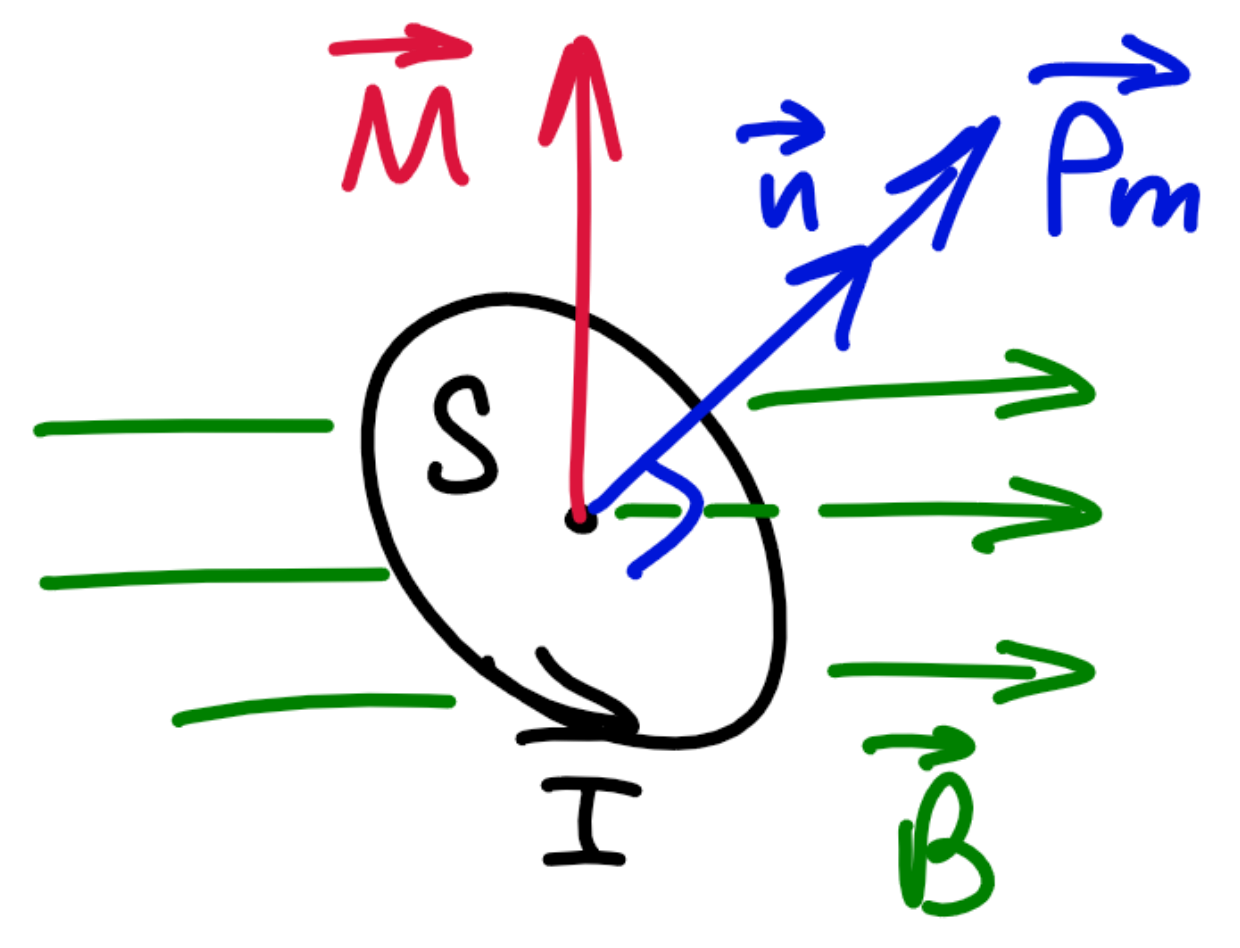
\includegraphics[width=0.25\textwidth]{graphics/19.png}
\end{center}
Рамка будет стремится ориентироваться так, чтобы в итоге $\vec{p_m}\upuparrows\vec{B}$
% ------------------------------------
\section{Сила Лоренца. Движение заряженных частиц в постоянном магнитном поле}
% --- --- ---
\subsection*{Сила Лоренца}
\textbf{Опр.} Сила, действующая на заряженную частицу со стороны
магнитного и электрического поля, называется
\[\textrm{\underline{\textit{силой Лоренца:}}} \ \vec{F_\textrm{Л}} =
    q\vec{E} + q\vec{\upsilon}\times\vec{B}\]
Часто под силой Лоренца подразумевается лишь магнитная её составляющая
$F_\textrm{Л} \approx q\vec{\upsilon}\times\vec{B}$
% --- --- ---
\subsection*{Движение заряженных частиц в постоянном магнитном поле}
\textit{\textcolor{BlueViolet}{Сила}} $F_\textrm{Л}$, оказываемая полем на частицу,
направлена перпендикулярно её движению. Следовательно, работу она не совершает,
а лишь искривляет траекторию движения.
\begin{center}
    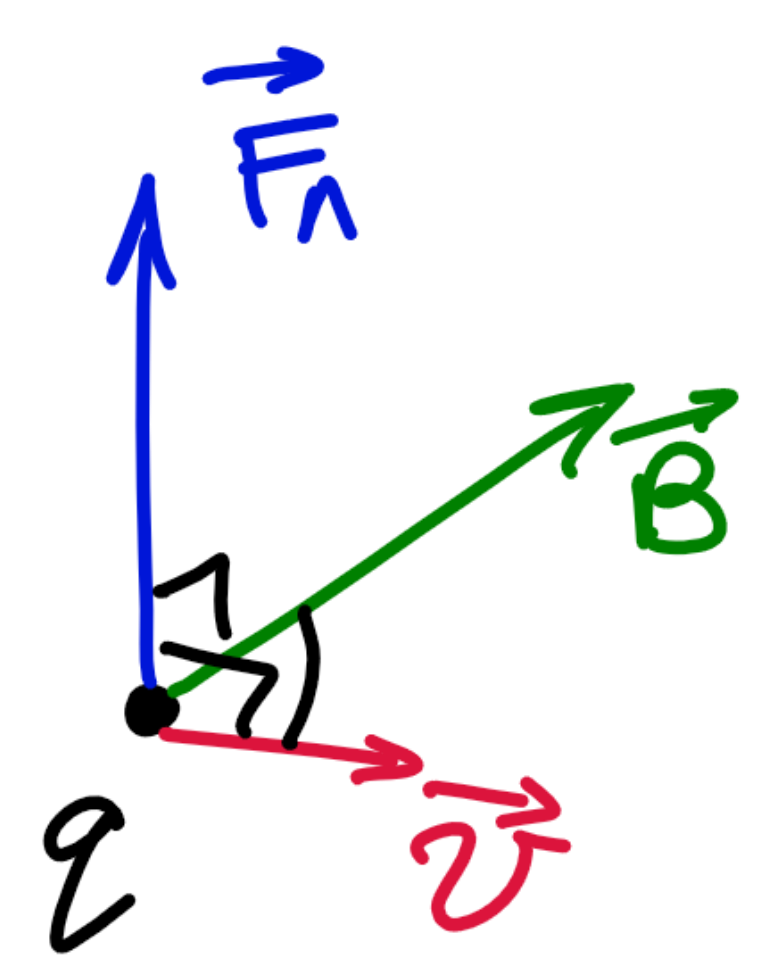
\includegraphics[width=0.175\textwidth]{graphics/20.png}
\end{center}
Принимая во внимание только магнитную составляющую, модуль силы Лоренца таким образом
$F_\textrm{Л} = q\upsilon B\sin{(\vec{\upsilon}, \vec{B})}$
% ------------------------------------
\section{Дифференциальная и интегральная формы записи уравнений магнитостатического поля в вакууме}
% --- --- ---
\subsection*{Словестная}
\begin{itemize}
    \item[] \underline{Теорема о потоке вектора магнитной индукции:}\\
        Магнитный поток сквозь произвольную замкнутую поверхность равен нулю.
        % ---
    \item[] \underline{Теорема о циркуляции вектора магнитной индукции:}\\
        Циркуляция вектора магнитной индукции по замкнутому контуру равна
        произведению суммы токов, пронизывающих контур, на магнитную постоянную.
\end{itemize}
% --- --- ---
\subsection*{Интегральная}
$\oint_S{\vec{B}\vec{dS}} = 0 \ \textrm{---} \ \mathbb{T} \
    \textrm{о потоке} \ \vec{B}$\\
$\textrm{\hspace{15pt}} \oint_L{\vec{B}\vec{dl}} = \mu_0\sum_{k = 1}^{n}{I_k}\ \textrm{---} \ \mathbb{T} \
    \textrm{о циркуляции} \ \vec{B}$
% --- --- ---
\subsection*{Дифференциальная}
$div\vec{B} = 0 \ \textrm{---} \ \mathbb{T} \
    \textrm{о потоке} \ \vec{B}$\\
$\textrm{\hspace{18pt}} rot\vec{B} = \mu_0\vec{\jmath}\ \textrm{---} \ \mathbb{T} \
    \textrm{о циркуляции} \ \vec{B}$
% ------------------------------------
\section{Описание магнитного поля в магнетиках. Намагничивание, магнитная восприимчивость и проницаемость. Напряженность магнитного поля. Ферромагнетизм. Диамагнетизм. Парамагнетизм}
% --- --- ---
\subsection*{Напряжённость магнитного поля}
\textbf{Опр.} Векторная физическая величина, количественно характеризующая магнитное поле
и не зависящая от магнитных свойств среды, называется
\textit{напряжённостью магнитного поля}.
Единица измерения --- ампер на метр,
[\textit{$\frac{\textrm{А}}{\textrm{м}}$}].

Напряжённость магнитного поля связана с индукцией: $\vec{B} = \mu_0\vec{H}$
% --- --- ---
\subsection*{Намагничивание, магнитная восприимчивость и проницаемость}
Попадая в магнитное поле, вещество намагничивается.
Причина этому --- молекулярное строение.
\begin{center}
    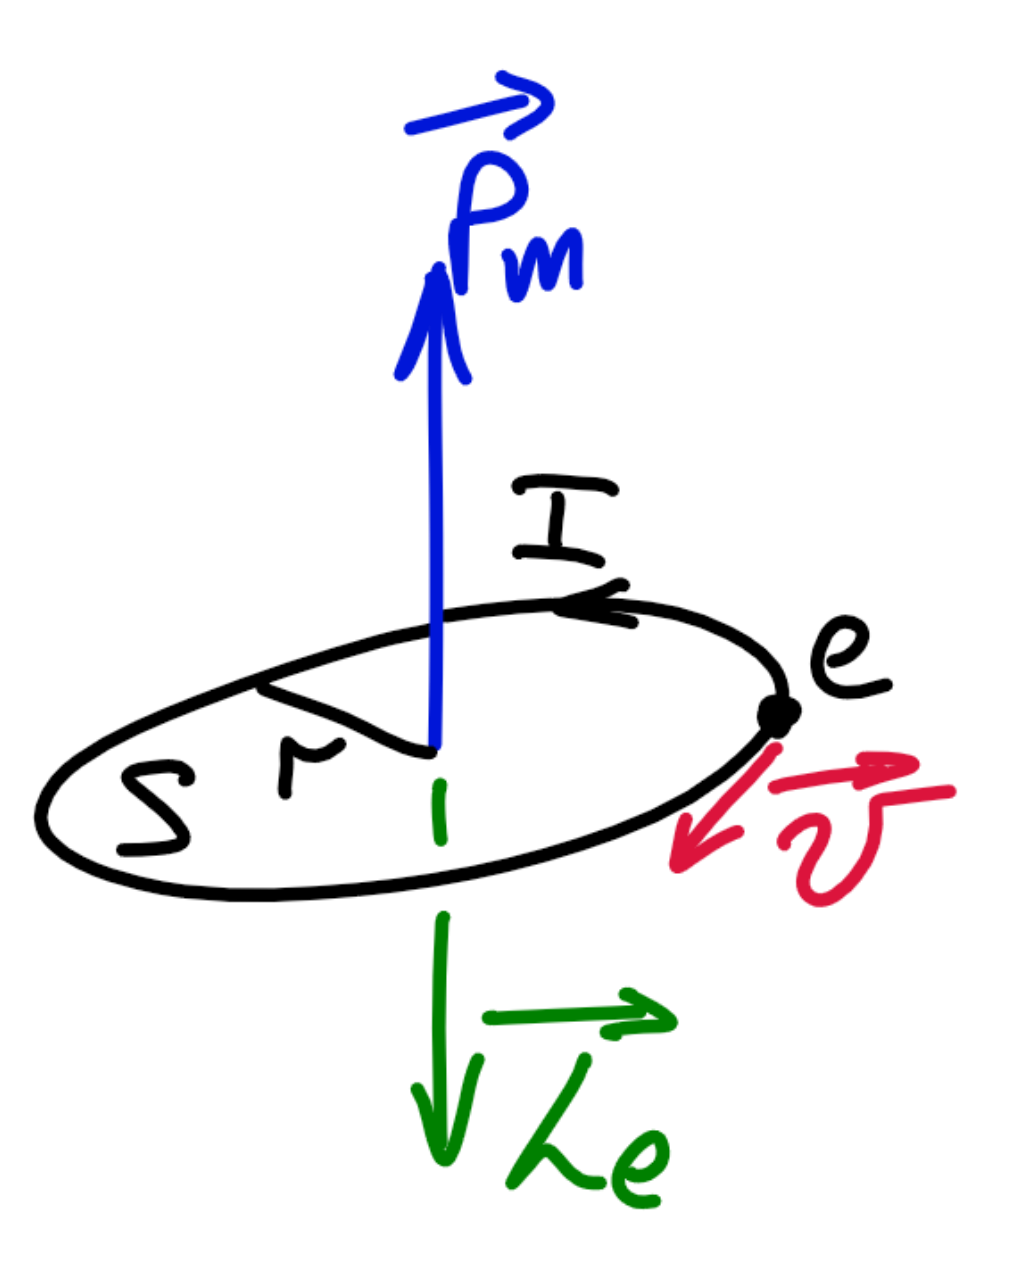
\includegraphics[width=0.2\textwidth]{graphics/22_1.png}
\end{center}
Рассмотрим \textit{\textcolor{BlueViolet}{магнитный момент}} электрона:
\[\vec{p_m} = IS\vec{n} \qquad p_m = e \upsilon S = e \frac{\upsilon}{2\pi r}\pi r^2 =
    \frac{1}{2}e\upsilon r \]
Помимо него, согласно механике, у электрона есть
\textit{\textcolor{OliveGreen}{момент имппульса}}:
\[\vec{L_e} = m\vec{\upsilon}\times\vec{r} \qquad L_e = m\upsilon r\]
Выражая из второго часть $\upsilon r$, получаем
\[ \vec{p_m} = \gamma\vec{L_e} \textrm{, где} \quad \gamma = \frac{e}{2m} \
    \textrm{--- гиромагнитное отношение.} \]

Зная магнитные моменты для молекул, можно рассчитать \textit{намагниченность} вещества:
\[\vec{J} = \frac{1}{\varDelta V} \sum_{i=1}^{n}\overrightarrow{{p_m}_i},
    \quad \textrm{где} \ \varDelta V \ \textrm{--- макроскопически малый объём.}\]
% --- --- ---
\subsection*{Описание магнитного поля в магнетиках}
Для для слабых полей и магнетиков, намагниченность выражается следующим образом:
$\vec{J} = \chi\vec{H}$, где $\chi$ --- магнитная восприимчивость (безразмерная).
% --- --- ---
\subsubsection*{1. Диамагнетизм}
--- намагничивание веществ навстречу направлению действия внешнего магнитного поля
(этим свойством обладают все вещества). Примеры: вода, золото, серебро.

Их магнитная восприимчивость $\chi$ отрицательна и имеет порядок около $10^{-6}$.
% --- --- ---
\subsubsection*{2. Парамагнетизм}
--- намагничиваение веществ в направлении действия внешнего магнитного поля. Примеры:
аллюминий, магний, натрий, калий, уран.

Такие вещества обладают собственным магнитным моментом $\vec{p_m}$,
а их магнитная восприимчивость $\chi$ положительна и имеет порядок около $10^5$.
% --- --- ---
\subsubsection*{3. Ферромагнетизм}
--- спонтанное намагничивание при температуре ниже точки Кюри и в отутствие внешнего
магнитного поля, при чём атомные магнитные моменты ферромагнетиков параллельны
друг другу.

Подобно сегнетоэлектрикам, обладают явлением \textit{гистерезиса} ---
из-за перераспределения очагов спонтанного намагничивания (доменов)
зависимость индукции от напряжённости становится неоднозначной, петлеобразной.
Возникает коэрцитивная сила, стремящаяся погасить остаточное намагничивание и
привести вещество обратно к состоянию насыщения:
\begin{center}
    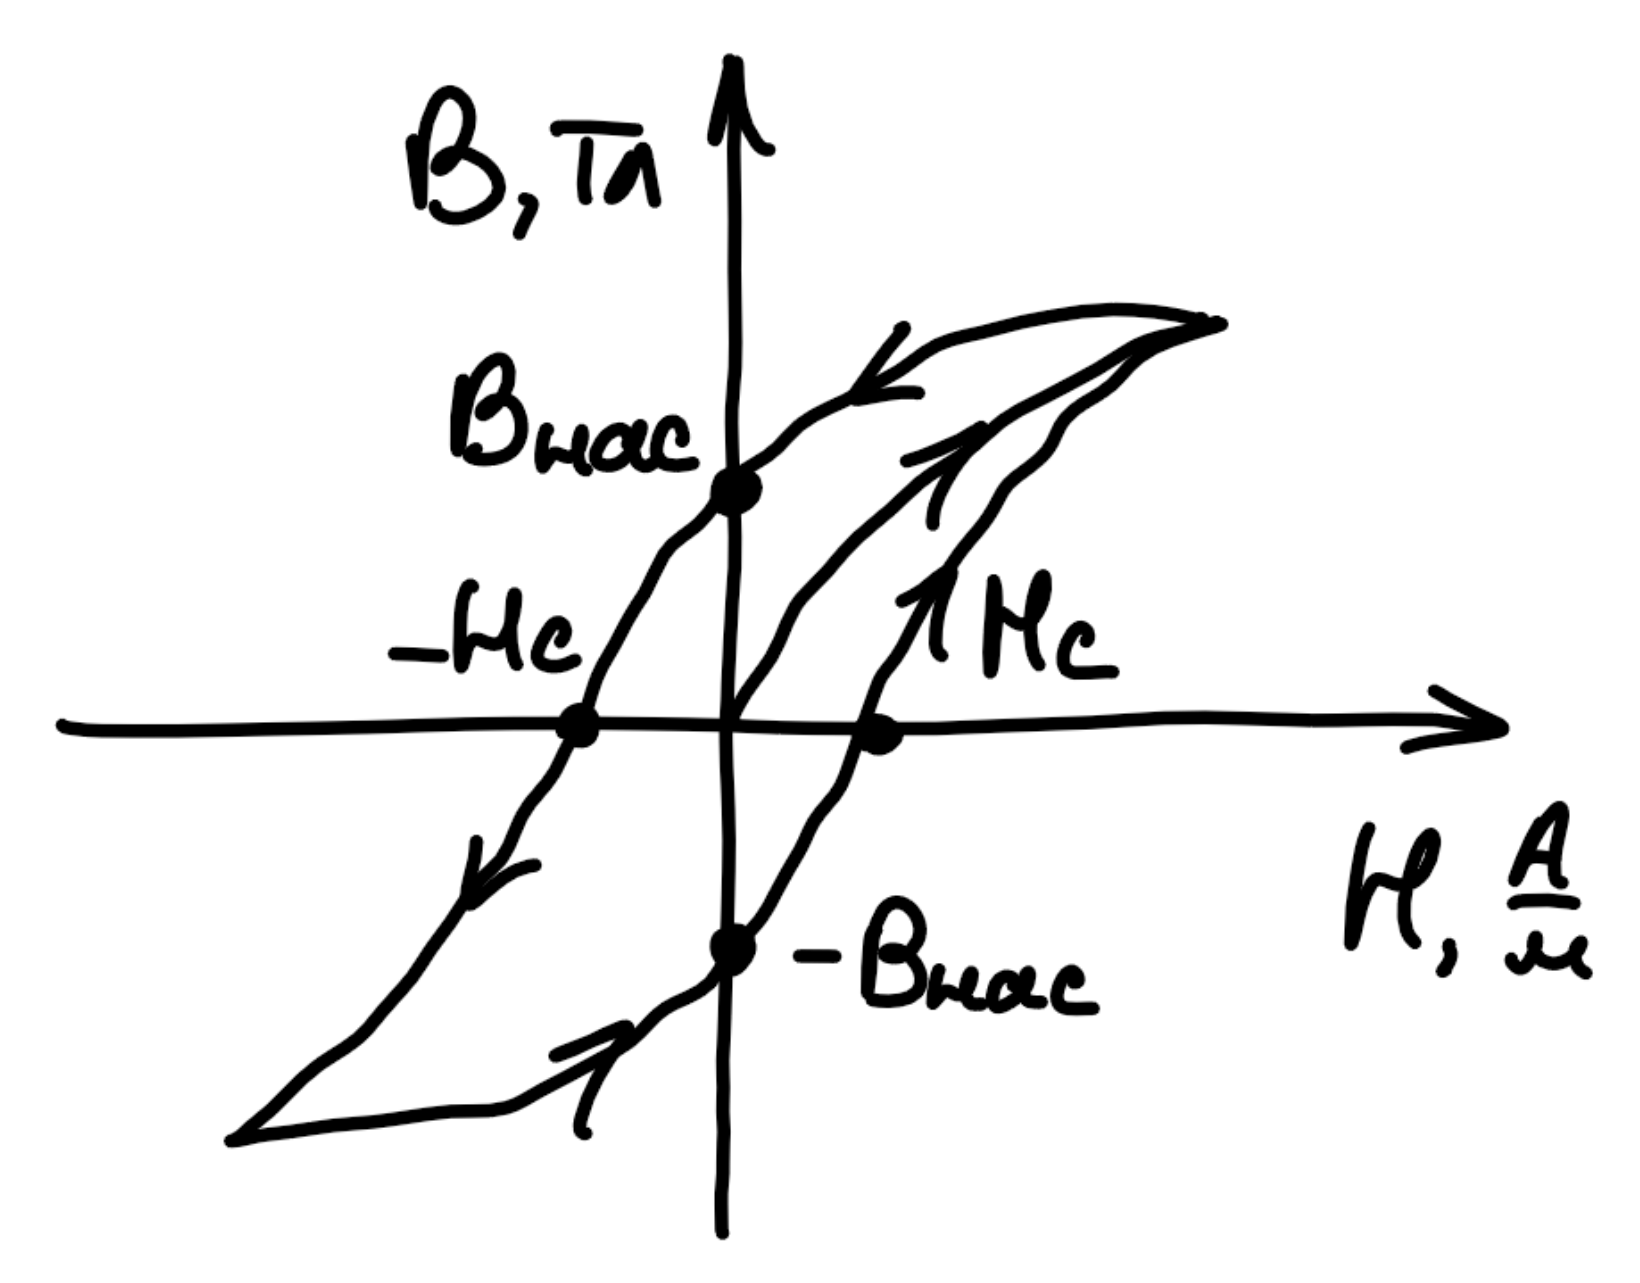
\includegraphics[width=0.325\textwidth]{graphics/22_2.png}
\end{center}

\subsubsection*{Отличия в намагниченности у магнетиков}
Наглядные различия между \textit{\textcolor{BlueViolet}{диамагнетиками}},
\textit{\textcolor{OliveGreen}{парамагнетиками}} и
\textit{\textcolor{BrickRed}{ферромагнетиками}}:
\begin{center}
    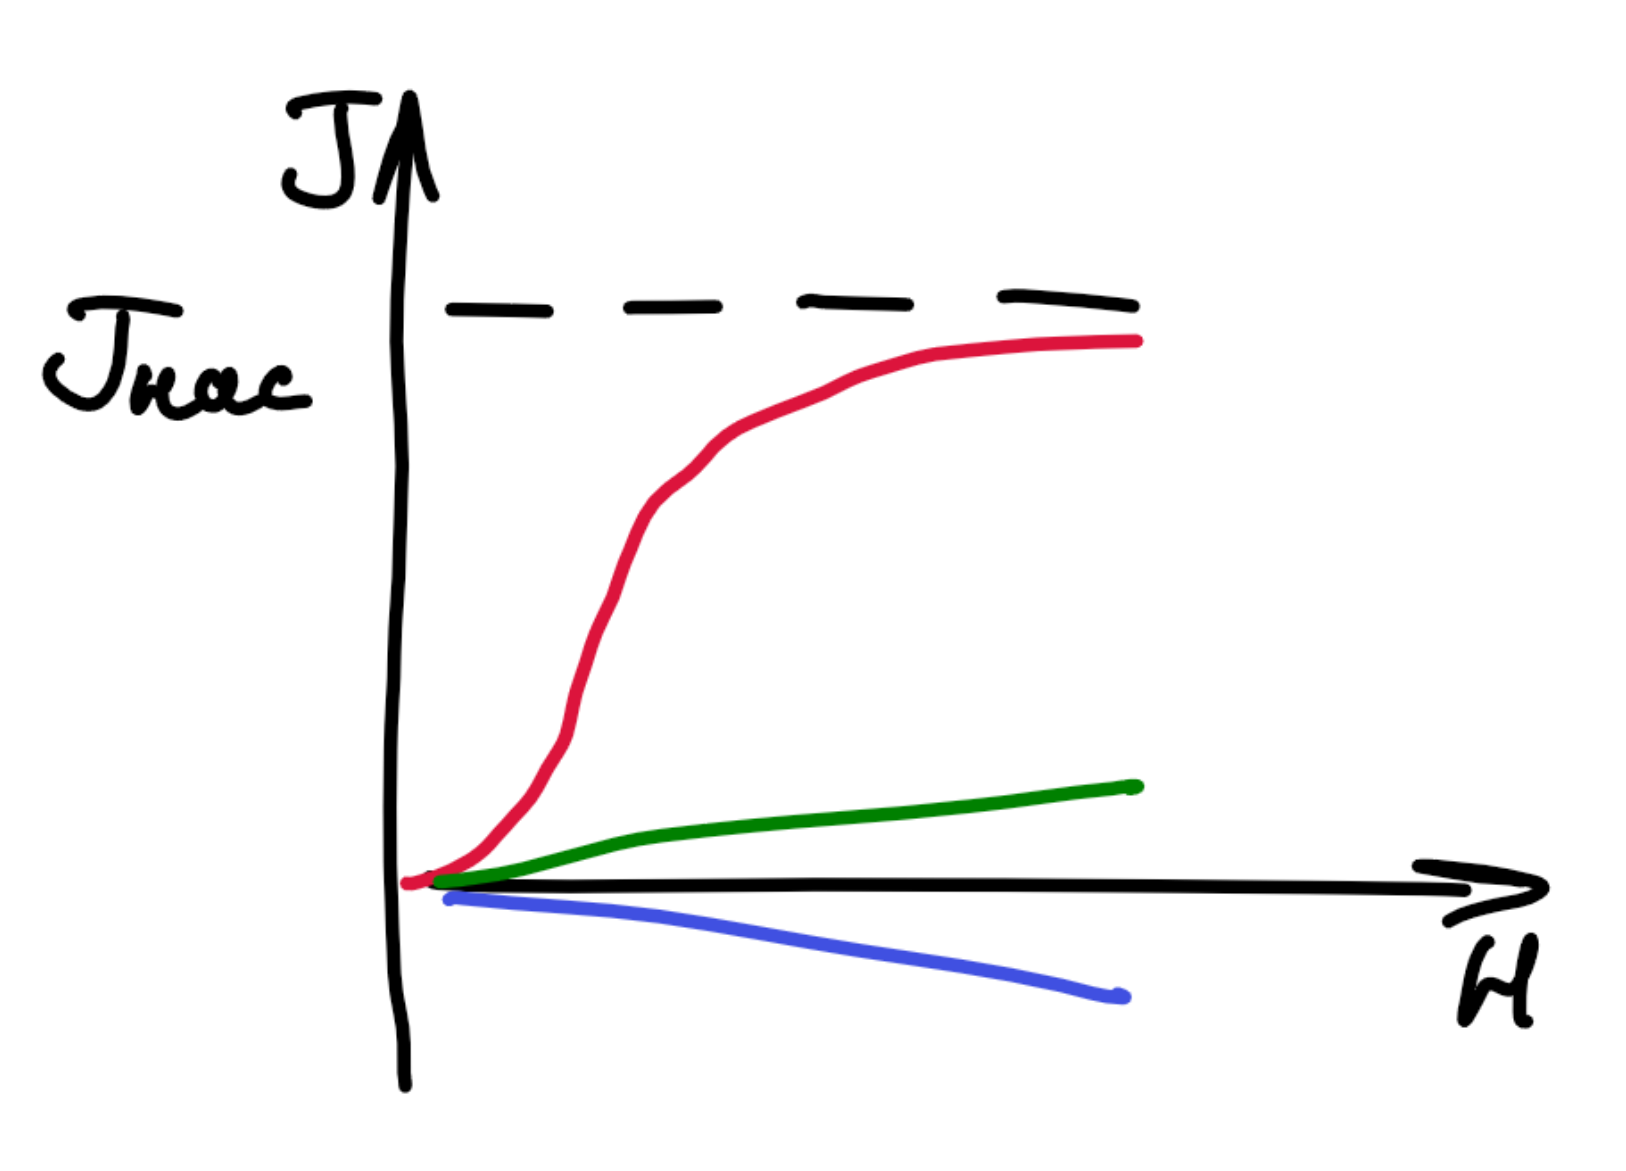
\includegraphics[width=0.325\textwidth]{graphics/22_3.png}
\end{center}
% ------------------------------------

\setcounter{section}{22}

\section{Электромагнитная индукция. Закон Фарадея. Правило Ленца. Вихревое электрическое поле.}
Электромагнитная индукция --- явление возникновения электрического тока в замкнутом контуре при изменении во времени магнитного потока.

Электромагнитная индукция --- возникновение электрич. поля, электрич. тока или электрич. поляризации при изменении во времени магн. поля или при движении материальных сред в магн. поле.

\subsection{Закон Фарадея}
ЭДС электромагнитной индукции в контуре численно равна и противоположна по знаку скорости изменения магнитного потока сквозь поверхность, натянутую на этот контур. ЭДС возникает, если поток $\Phi_B$ изменяется по любым причинам.
\[
    \varepsilon_i = - \dfrac{\dd{\Phi_B}}{\dd t}
\]

\subsection{Правило Ленца}
При всяком изменении магнитного потока сквозь поверхность, натянутую на замкнутый проводящий контур, в последнем возникает индукционный ток такого направления, что его магнитное поле противодействует изменению магнитного потока.

\subsection{Вихревое электрическое поле}
Возникновение ЭДС электромагнитной индукции и индукционного тока в неподвижном проводящем контуре, находящемся в переменном магнитном поле, нельзя объяснить действием на носители тока магнитной составляющей силы Лоренца, т.к. на неподвижные заряды эта сила не действует.

Максвелл предположил, что изменение магнитного поля вызывает появление вихревого электрического поля, и это поле приводит к появлению $\varepsilon_i$.
\[
    \oint_l \vec{E} \dd{\vec{l}} = -\dfrac{\dd{\Phi_B}}{\dd{t}}
\]

\section{Энергия магнитного поля}
Энергия магнитного поля показывает, какую работу затратил электрический ток в проводнике (катушке индуктивности) на создание этого магнитного поля:
\[
    E = \dfrac{L I^2}{2}
\]
Где $L$ --- индуктивность, $I$ --- сила тока.

\setcounter{section}{29}
\section{ПОЛЯРИЗАЦИЯ СВЕТА. Естественный и поляризованный свет. Cтепень поляризации света. Поляризация при отражении и преломлении. Закон Брюстера. Двойное лучепреломление. Поляроиды и поляризационные призмы. Закон Малюса.}
\subsection{  Естественный и поляризованный свет.}
\textbf{Естественный свет} - совокупность электромагнитных волн со всевозможными равновероятными направлениями световых векторов (напряженности электрического поля $\overrightarrow{E}$), перпендикулярных направлению распространения света.

\textbf{Поляризованный свет} -  Поляризованным светом называется свет, в котором направления колебания вектора напряженности электрического поля $\overrightarrow{E}$  каким-либо образом упорядочены.
\subsection{  Cтепень поляризации света.}
Степень выделения световых волн с определённой ориентацией векторов напряжённости электрического и магнитного полей;
\[P=\frac{I_{max}-I_{min}}{I_{max}+I_{min}}\]
Где $I_{max}$ и $I_{min}$ - наибольшая и наименьшая интенсивности света, прошедшие через поляризатор при разных его положениях.\\
$P=0$ - Для естественного света и круговой поляризации, $I_{max}=I_{min}$.\\
$0<P<1$ - Для частичной поляризации.\\
$P=1$ - Для  линейной поляризации света и круговой поляризации,  $I_{min}=0$.
\subsection{  Поляризация при отражении и преломлении.}
При отражении от проводящей поверхности (металлического зеркала) получается эллиптически-поляризованный свет.\\
При падении света на границу раздела двух диэлектриков (например, из воздуха на поверхность стеклянной пластинки) под углом отличным от нуля, отражённый и преломлённый лучи оказываются частично поляризованными. В отражённом луче преобладают колебания, перпендикулярные к плоскости падения, в преломлённом луче – колебания, параллельные плоскости падения.
\subsection{  Закон Брюстера.}
При падении света под углом Брюстера преломленные лучи оказываются частично поляризованными.\\

Если свет падает на границу раздела под углом Брюстера, то отраженный и преломленный лучи взаимно перпендикулярны.

\begin{center}
    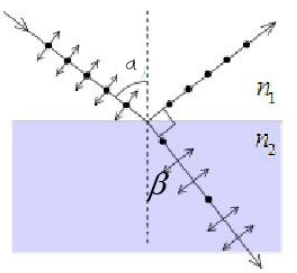
\includegraphics[scale=0.7]{graphics/30_1.png}
\end{center}

\[ \frac{sin(\alpha_{Br})}{sin(\beta)} = \frac{n_2}{n_1} \Rightarrow{}  \alpha_{Br}+\beta = \frac{\pi}{2} \]  \[ sin(\beta) = sin(\alpha_{Br} - \frac{\pi}{2}) \Rightarrow{} sin(\beta) = cos(\alpha_{Br}) \Rightarrow{} \frac{sin(\alpha_{Br})}{sin(\beta)} =
    \frac{sin(\alpha_{Br})}{cos(\alpha_{Br})} = tg(\alpha_{Br})=\frac{n_2}{n_1}\]\\
$tg(\alpha_{Br})=\frac{n_2}{n_1}$ - соотношение при угле Брюстера
$n_1$ и $n_2$ - показатели преломления сред.
\subsection{  Двойное лучепреломление.}
\textbf{Двойное лучепреломление} - раздвоение светового луча при прохождении через анизотропную среду, обусловленное зависимостью показателя преломления (а следовательно, и скорости волны) от её поляризации и ориентации волнового вектора относительно кристаллографич. осей, т.е. от направления распространения.\\

Направление в оптически анизотропном кристалле, по которому луч света не испытывает двойного лучепреломления, называется оптической \textbf{осью кристалла}.\\

Главная плоскость, или главное сечение, одноосного кристалла для какого-либо луча называется плоскость, проходящая через этот луч и
пересекающая его оптическую ось.\\
\subsection{ Поляроиды и поляризационные призмы.}
\textbf{Поляризационные призмы} - один из классов призм оптических, простейшие поляризационные приборы, предназначенные для получения линейно поляризованного оптического излучения (см. Поляризация света) или для определения характера и степени его поляризации. В соответствии с этим поляризационные призмы в оптических приборах выполняют функции поляризаторов или анализаторов.\\

\textbf{Поляроиды}-то прозрачные пленки, поляризующие свет, светофильтры, пропускающие только такие световые колебания, которые совершаются в одном определенном направлении, перпендикулярном к лучу. Две пленки, наложенные друг на друга, пропускают свет, если направления колебаний в них совпадают, и не пропускают света, если эти направления скрещены.
\subsection{ Закон Малюса.}
\textbf{Закон Малюса} - зависимость интенсивности линейно поляризованного света после его прохождения через анализатор от угла $\varphi$ между лоскостями поляризации падающего света и анализатора.

\begin{center}
    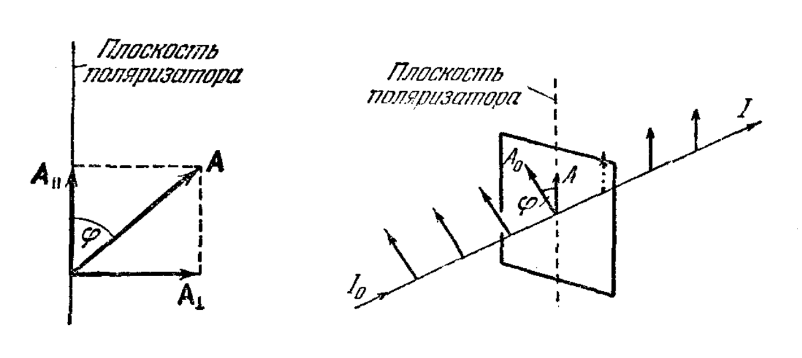
\includegraphics[scale=0.7]{graphics/30_2.png}
\end{center}

\[
    I=I_0*cos^2(\varphi)
\]
$I_0$ - интенсивность плоскополяризованного
света, падающего на анализатор.\\
$I$ -интенсивность света, вышедшего из
анализатора\\
Свет с иной (не линейной) поляризацией может быть
представлен в виде суммы двух линейно поляризованных
составляющих, к каждой из которых применим закон Малюса.

Прохождение естественного света через поляризатор:\\
Так как среднее значение $cos^2(\varphi)$=$\frac{1}{2}$ то интенсивность поляризованного света равна половине интенсивности естественного света.
\[
    I_\text{п}=\frac{1}{2} \cdot I_0
\]
Прохождение естественного света через два поляризатора:\\
\[
    I=I_0*cos^2(\varphi), I_0=\frac{1}{2}\cdot I_\text{ест} \Rightarrow{} I=\frac{1}{2}\cdot I_\text{ест} \cdot cos^2(\varphi)
\]
\section{КВАНТОВЫЕ СВОЙСТВА СВЕТА. Внешний фотоэффект и его законы. Уравнение Эйнштейна для фотоэффекта. Красная граница фотоэффекта. Фотоны. Энергия, масса и импульс фотона. Эффект Комптона и его теория. Давление света.}
\subsection{ Внешний фотоэффект и его законы.}
\textbf{Фотоэффект} - испускание электронов веществом при поглощении им квантов электромагнитного излучения (фотонов).

\textbf{Внешним фотоэффектом} - называется испускание
электронов веществом под действием электромагнитного
излучения.\\

\textbf{Внутренний фотоэффект} – возникновение свободных
носителей заряда - электронов и (или) дырок - в твёрдом
теле при поглощении в нём квантов электромагнитного
излучения (фотонов).\\

\textbf{Вентильный фотоэффект} - возникновение ЭДС (фото-
ЭДС) при освещении контакта двух разных полупроводников или полупроводника и металла (при отсутствии внешнего электрического поля).

\subsubsection{Законы:}
Закон Столетова: при фиксированной частоте падающего света число фотоэлектронов, вырываемых из катода в единицу времени, пропорционально интенсивности света (фототок насыщения пропорционален энергетической освещенности катода).

Максимальная скорость фотоэлектронов не зависит от интенсивности падающего света, а определяется только его частотой ν.

Для каждого вещества существует красная граница фотоэффекта, т.е. минимальная частота $v_0$ света (зависящая от химической природы вещества и состояния его поверхности), ниже которой фотоэффект невозможен: $v_\text{кр}=\frac{A}{h}$\\
$A$ - работа выхода.\\
$h$ - постоянная Планка.
\subsection{ Уравнение Эйнштейна для фотоэффекта.}
Свет не только испускается (Планк), но и распространяется, и поглощается веществом отдельными порциями (квантами), энергия которых: $ E = h\nu $\\
\[E=h\nu=A_вых+\frac{m*v^2}{2}\]

Максимальное значение тока $I_н$ – фототок насыщения – определяется
таким значением $U_z$, при котором все электроны, испускаемые катодом, достигают анода.\\
\[\frac{m*v_{max}^2}{2}=eU_z \Rightarrow{} E=h\nu=A_вых+eU_z\]
$A_вых$ - \textbf{работа выхода} - энергия, которая затрачивается
твёрдым или жидким телом при тепловом
возбуждении электрона этого тела в вакуум (в
состояние с кинетич. энергией равной нулю).\\

$U_z$ - задерживающее напряжение.\\

$e$ - элементарный заряд(электрон).\\

$h$ - постоянная Планка.\\

$\nu = \dfrac{c}{\lambda}$ - частота.\\

$c$ - скорость света.\\

$\lambda$ - длина волны.\\

$v$ - скорость заряда(электрона).\\

$m$ - масса элементарного заряда(электрона).\\

$\dfrac{m \cdot v^2}{2}$ - кинетическая работа фотоэффекта.
\subsection{Красная граница фотоэффекта.}
Красная граница фотоэффекта – минимальная частота света, ниже которой фотоэффект невозможен (красная граница фотоэффекта зависит от химической природы вещества и состояния его поверхности).\\
Красной границей фотоэффекта также называют максимальную длину волны света, выше которой фотоэффект невозможен.
\subsection{Фотоны.}
\textbf{Фотон} -элементарная частица, квант эл/магн. поля.\\
Излучается порция энергии (квант): $E=h\nu=h\dfrac{c}{\lambda}$\\
Все фотоны в вакууме всегда движутся с одной и той же
скоростью света $с$ = 3·108 м/с.
\subsection{Энергия, масса и импульс фотона.}

$E=mc^2$ и $E=h\nu=\dfrac{hc}{\lambda}$ - энергия\\

$m=\dfrac{h\nu}{c^2}=\dfrac{h}{c\lambda}$ - масса\\

$p=\dfrac{h}{\lambda}=\dfrac{h\nu}{c}=\dfrac{h_1\omega}{c}=h_1k$ - импулься\\

$\omega=2\pi\nu$ - угловая частота волны.\\

$h_1 = \dfrac{h}{2\pi}$ - одна из записей постоянной Планка.\\

$k=\dfrac{\omega}{c}$ - волновое число.
\subsection{ Эффект Комптона и его теория.}
Рассеяние эл-магн. волны на свободном электроне, сопровождающееся
уменьшением частоты. Столкновение квантов света – фотонов с
электронами приводит к эффекту Комптона. Эффект наблюдается для больших частот рассеиваемого эл-магн. излучения (в рентг. области и выше).\\

$\Delta\lambda = \lambda_c(1-\cos(\alpha))$-формула Комптона.
Значение постоянной $\lambda_c = 2,426*10^{−12}$ \\

$h_1=\dfrac{h}{2\pi}$\\
Закон сохранения энергии:
$h_1\dfrac{2c\pi}{\lambda}+m_ec^2=h_1\dfrac{2c\pi}{\lambda^{'}}+E_e$\\
Закон сохранения импульса:
$h_1\overrightarrow{k}=h_1\overrightarrow{k^{'}} + m\overrightarrow{v}$, $k=\dfrac{2\pi}{\lambda}$\\

$\lambda^{'}-\lambda = \dfrac{h}{m_ec} (1-\cos(\alpha))$ - Закон изменения длины волны при эффекте
Комптона
\subsection{ Давление света.}
Световое излучение оказывает давление на
материальные предметы, причем величина давления
пропорциональна интенсивности излучения\\

$p=\dfrac{I}{c}(1+R)$ - \\

$I=hn\lambda$ - интенсивность света.\\

$n$ - число фотонов, падающих в единицу времени на единицу
площади.\\

$R$ - коэффициент отражения света от поверхности.

\chapter{Задачи}
\section{Расчет напряженности и потенциала электрического поля тонкого равномерно заряженного отрезка прямой на линии, продолжающей отрезок (на перпендикуляре, восстановленном к середине отрезка; на перпендикуляре, восстановленном к одному из концов отрезка и т.п.)}
Пусть $k = \dfrac{1}{4\pi \varepsilon_0 \varepsilon}$. Тогда:
\[
    \vec{E} = k\dfrac{q\vec{r}}{\abs{\vec{r}}^3} \ \Rightarrow\ \begin{cases}
        E_x = \abs{\vec{E}} \cos{\alpha} = k\dfrac{q}{r^2} \cos{\alpha} \\
        E_y = \abs{\vec{E}} \sin{\alpha} = k\dfrac{q}{r^2} \sin{\alpha}
    \end{cases}
\]

Дано:
\begin{itemize}
    \item $L$ --- длина отрезка
    \item $a$ --- кратчайшее расстояние до отрезка
    \item $\tau$ --- линейная плотность заряда на отрезке
\end{itemize}

Расположим отрезок и оси координат так, чтобы точка, для которой проводятся измерения, оказалась в центре, а отрезок --- вертикально в первой четверти (другие случаи рассмотрим позднее):

\begin{center}
    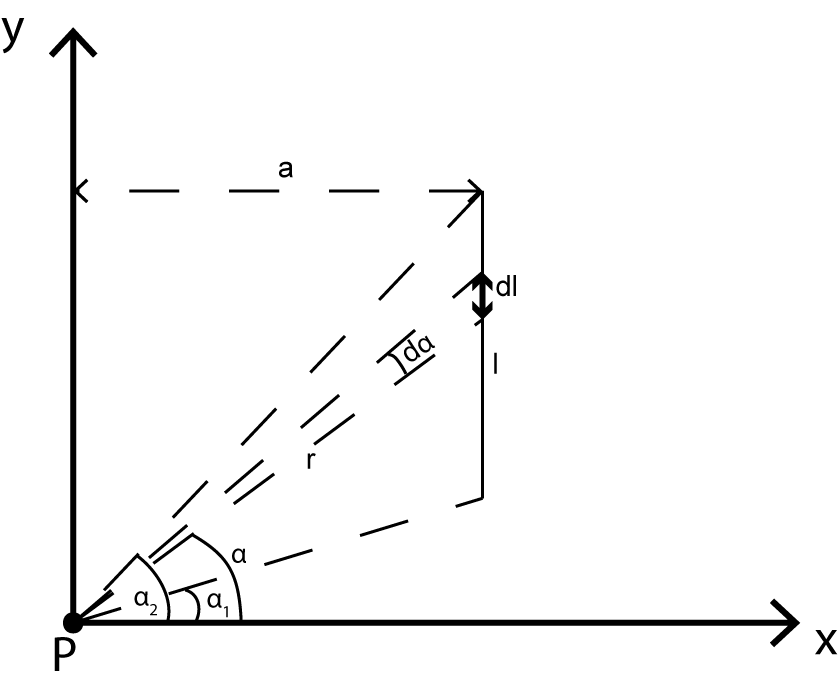
\includegraphics[width=0.5\textwidth]{graphics/t01.png}
\end{center}

Пусть $\alpha_1 < \alpha_2$.

\begin{align*}
     & l = a\tan \alpha                            \\
     & \dd l = \dfrac{a }{\cos^2 \alpha}\dd \alpha \\
     & r = \dfrac{a}{\cos \alpha}                  \\
\end{align*}

Нам дана линейная плотность заряда отрезка $\tau$. Возьмём бесконечно малую часть отрезка $\dd l$. Её заряд: $\dd q = \tau \dd l$.

Тогда напряжённость и потенциал от неё будут:
\[
    \dd \vec{E} = k \dfrac{\dd q \vec{r}}{\abs{\vec{r}}^3} = k \dfrac{\tau \vec{r} \dd l}{\abs{\vec{r}}^3}
    \\
    \dd \phi = k \dfrac{\tau \vec{r} \dd l}{\abs{\vec{r}}^2}
\]

Разобьём $\vec E$ на две составляющих: $E_x$ и $E_y$. Тоже самое проделаем с потенциалом. Тогда:
\begin{align*}
     & \dd {E_x} = -k \dfrac{\tau \cos^2 \alpha}{a^2} \cdot \dfrac{a}{\cos^2 \alpha} \dd \alpha \cdot \cos{\alpha} = k \dfrac{\tau \cos{\alpha}}{a}\dd \alpha \\
     & \dd {E_y} = -k \dfrac{\tau \sin{\alpha}}{a}\dd \alpha                                                                                                  \\
     & E_x = -\dfrac{k \tau}{a}\int_{\alpha_1}^{\alpha_2} \cos{\alpha}\dd \alpha = \dfrac{k \tau}{a}(\sin{\alpha_1} - \sin{\alpha_2})                         \\
     & E_y = -\dfrac{k \tau}{a}\int_{\alpha_1}^{\alpha_2} \sin{\alpha}\dd \alpha = \dfrac{k \tau}{a}(\cos{\alpha_2} - \cos{\alpha_1})                         \\
     & \dd {\phi_x} = k \dfrac{\tau \cos \alpha}{a} \cdot \dfrac{a}{\cos^2 \alpha} \dd \alpha \cdot \cos{\alpha} = k\tau\dd \alpha                            \\
     & \dd {\phi_y} = k \tau \tan{\alpha}\dd \alpha                                                                                                           \\
     & \phi_x = k\tau(\alpha_2 - \alpha_1)                                                                                                                    \\
     & \phi_y = k\tau(\log|\cos \alpha_1| - \log|\cos \alpha_2|) = k \tau \log\vqty{\dfrac{\cos \alpha_1}{\cos \alpha_2}}                                     \\
     & \phi = \sqrt{\phi_x^2 + \phi_y^2} = k\tau\sqrt{(\alpha_2 - \alpha_1)^2 + \log^2\vqty{\dfrac{\cos \alpha_1}{\cos \alpha_2}}}
\end{align*}

Случай, когда отрезок и точка находятся на одной прямой тривиален --- там меняется только расстояние:
\[
    |\vec{E}| = k\tau \int_{r_1}^{r_2}\dfrac{dr}{r^2} = k\tau\left(\dfrac{1}{r_1} - \dfrac{1}{r_2}\right)
\]

\section{Расчет напряженности и потенциала электрического поля на оси тонкого равномерно заряженного кольца.}
\begin{center}
    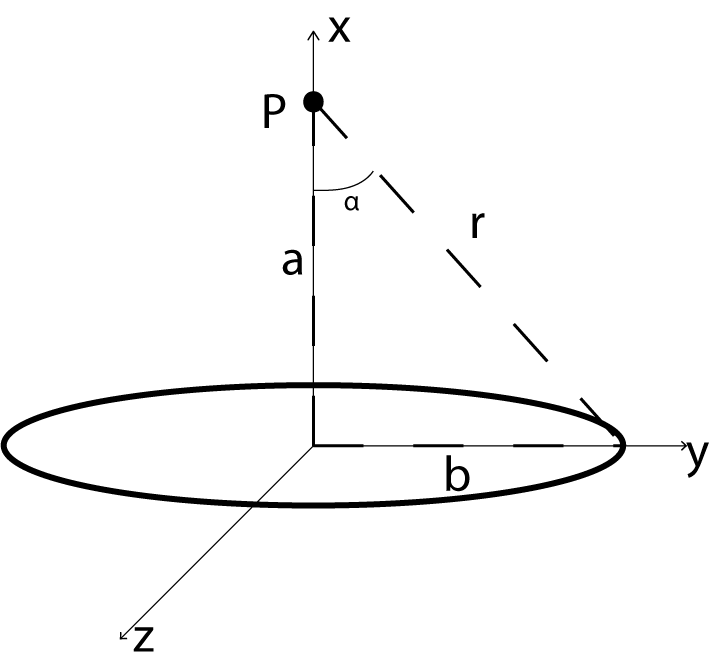
\includegraphics[width=0.5\textwidth]{graphics/t02.png}
\end{center}
Очевидно, что напряжённость по осям $y$ и $z$ скомпенсируют друг друга. Тогда:
\[
    E = \tau 2\pi b \dfrac{1}{4\pi \varepsilon\varepsilon_0 r^2} \cos \alpha
    = \dfrac{\tau b}{2\varepsilon\varepsilon_0 r^2} \cos \alpha
    = \dfrac{\tau ab}{2\varepsilon\varepsilon_0 r^3}
    = \dfrac{\tau ab}{2\varepsilon\varepsilon_0 \sqrt{(a^2 + b^2)^3}}
\]

Потенциал:
\[
    \phi = \tau 2\pi b \dfrac{1}{4\pi \varepsilon\varepsilon_0 r}
    = \dfrac{\tau b}{2\varepsilon\varepsilon_0 r}
    = \dfrac{\tau b}{2 \varepsilon \varepsilon_0 \sqrt{a^2 + b^2}}
\]

\section{Расчет напряженности и потенциала электрического поля в центре кривизны тонкого равномерно заряженного полукольца (дуги)}
\begin{center}
    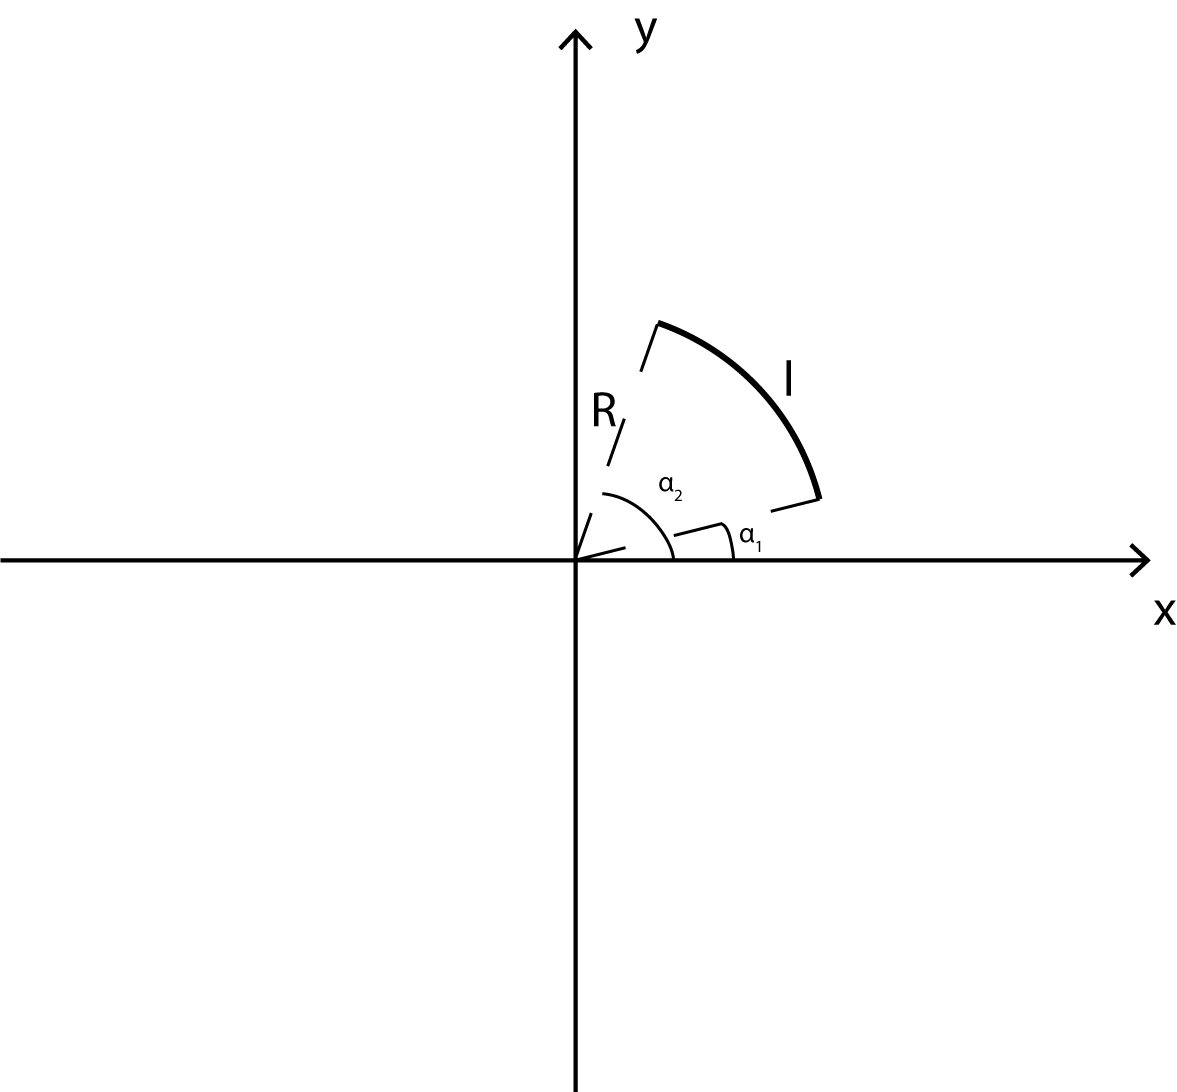
\includegraphics[width=0.5\textwidth]{graphics/t03.png}
\end{center}

Пусть $\alpha_1 < \alpha_2$.

\begin{align*}
     & l = 2\pi R \dfrac{\alpha_2 - \alpha_1}{2\pi} = R(\alpha_2 - \alpha_1)                          \\
     & \dd l = l \dfrac{\dd \alpha}{\alpha_2 - \alpha_1} = R \dd \alpha                               \\
     & \dd \vec E = \dfrac{\tau \vec{r} \dd \alpha}{4 \pi \varepsilon \varepsilon_0 R}                \\
     & \dd E_x = -\dfrac{\tau \dd \alpha}{4 \pi \varepsilon \varepsilon_0 R} \cos \alpha              \\
     & \dd E_y = -\dfrac{\tau \dd \alpha}{4 \pi \varepsilon \varepsilon_0 R} \sin \alpha              \\
     & k = \dfrac{\tau}{4\pi \varepsilon \varepsilon_0 R}                                             \\
     & E_x = -k \int_{\alpha_1}^{\alpha_2} \cos \alpha \dd \alpha = k (\sin \alpha_1 - \sin \alpha_2) \\
     & E_y = -k \int_{\alpha_1}^{\alpha_2} \sin \alpha \dd \alpha = k (\cos \alpha_2 - \cos \alpha_1) \\
\end{align*}

Потенциал (универсален):
\[
    \phi = \dfrac{l \tau}{4\pi \varepsilon\varepsilon_0 R}
    = \dfrac{(\alpha_2 - \alpha_1)\tau}{4\pi \varepsilon\varepsilon_0}
\]

\setcounter{section}{6}
\section{Напряженность электрического поля и потенциал шара, однородно заряженного о объему. Расчет разности потенциалов между центром и поверхностью равномерно заряженного однородного шара.}

Однородно заряженный шар. Пусть радиус шара R, полный заряд Q. Вне шара напряженность и потенциал поля совпадают с полем заряда Q, помещенного в центр шара:
\begin{center}
    $ E = k \frac{Q}{r^2} $, $ \varphi = k \frac{Q}{r} $
\end{center}
Чтобы найти напряженность электрического поля внутри шара, выберем в качестве замкнутой поверхности сферу радиуса r < R с центром в центре шара. Из симметрии ясно, что напряженность поля направлена по радиусу и одинакова по величине на всей поверхности сферы. Из теоремы Гаусса следует
\begin{center}
    $E(r) \cdot 4 \pi r^2 = 4 \pi kq(r)$
\end{center}
где q(r) – заряд внутри выбранной поверхности. Введем плотность заряда шара $\rho$. Тогда
\begin{center}
    $q(r) = \rho \frac{4}{3} \pi r^3$ и $E(r) = k \frac{q(r)}{r^2} = \frac{4}{3} \rho k r$
\end{center}
Плотность заряда равна полному заряду, деленному на объем шара:
\begin{center}
    $\rho = \frac{Q}{4 \pi R^3/3}$
\end{center}
Для напряженности поля внутри шара получим
\begin{center}
    $E = k\frac{Q}{R^3}r$
\end{center}
Найдем потенциал внутри шара.
\begin{center}
    $\varphi(r) = -\int_{\infty}^{r}  E\,dr = -\int_{\infty}^{R} k \frac{Q}{r^2}\,dr - \int_{R}^{r} k \frac{Q}{R^3}r \,dr $
\end{center}
Первый интеграл имеет смысл работы по переносу единичного положительного заряда из бесконечности до поверхности шара и равен kQ/R. Второй член
\begin{center}
    $-\int_{R}^{r} k \frac{Q}{R^3}r \,dr = -k \frac{Q}{R^3} \frac{r^2}{2} + k \frac{Q}{R^3} \frac{R^2}{2} $
\end{center}
Значение потенциала внутри шара определится выражением
\begin{center}
    $\varphi(r) = \frac{3}{2} k \frac{Q}{R} - k \frac{Qr^2}{2R^3}$
\end{center}
Окончательно имеем
\begin{center}
    $E = k \frac{q}{r^2}$, при r > R, $E = k \frac{Q}{R^3}r$, при r < R
\end{center}
\begin{center}
    $\varphi = k \frac{q}{r}$, при r > R, $\varphi = \frac{3}{2} k \frac{q}{R} - k \frac{Q}{2r^3}r^2$, при r < R
\end{center}
\newpage
\section{Напряженность и потенциал электрического поля\\ однородно заряженной сферы.}
Применим теорему Гаусса. Выберем в качестве замкнутой поверхности концентрическую сферу радиуса r > R (рис.). Очевидно, что напряженность на поверхности этой сферы будет одинакова по величине и направлена по радиусу. Тогда поток напряженности через нее будет $E \cdot 4\pi r^2$. Согласно теореме Гаусса
\begin{center}
    $E \cdot 4 \pi r^2 = 4 \pi k q$, откуда
\end{center}
\begin{center}
    $E = k \frac{q}{r^2}$
\end{center}
\par Выбрав в качестве поверхности сферу радиуса r < R, получим $E = 0$.
Таким образом, однородно заряженная сфера во внешней области пространства
создает такое же поле, как и заряд, помещенный в ее центре.
Внутри сферы поля нет.

Найдем потенциал сферы во всем пространстве.
Так как вне сферы напряженность поля совпадает с напряженностью заряда,
находящегося в центре, то и потенциал при r > R выразится в виде
\begin{center}
    $\varphi(r) = k \frac{q}{r}$
\end{center}
Пронесем единичный положительный заряд из бесконечности до расстояния r от центра,
меньшего радиуса сферы.
Тогда работа, которую необходимо совершить по переносу
до поверхности сферы будет равна kq/R.
Внутри сферы поле равно нулю и работа не совершается. Таким образом
\begin{center}
    $E = k \frac{q}{r^2}$ при $r > R, E = 0$ при $r < R$,
\end{center}
\begin{center}
    $\varphi = k \frac{q}{r}$ при $r > R$, $\varphi = k \frac{q}{R}$ при r < R.
\end{center}
\section{Напряженность и потенциал электрического поля бесконечного цилиндра, однородно заряженного по объему.}
Чтобы найти поле $E$ внутри заряженного цилиндра рассмотрим применение теоремы Гаусса к соосному цилиндру с радиусом $r \leq R$ и длиной $l$. $\rho$ --- объемная плотность заряда.
\begin{center}
    $\Phi_E = 4 \pi Q$
\end{center}
\begin{center}
    $ES = 4 \pi \rho V$
\end{center}
\begin{center}
    $E 2\pi r l = 4 \pi \rho \pi r^2 l$
\end{center}
\begin{center}
    $E = 2 \pi \rho r$, при $r \leq R$
\end{center}
\par Потенциал:
\begin{center}
    $W_p = \frac{q_0 Q}{4 \pi \varE_0 r}$
\end{center}
\begin{center}
    $\varphi = \frac{W_p}{q_0} = \frac{Q}{4 \pi \varE_0 r}$
\end{center}
\begin{center}
    $\varphi = \frac{\rho \pi r^2 l}{4 \pi \varE_0 r} $
\end{center}
\begin{center}
    $\varphi = \frac{\rho r l}{4 \varE_0}$
\end{center}
Найдем теперь поле $\vec{E}$ снаружи заряженного цилиндра при $r \geq R$.
Рассмотрим цилиндр с радиусом $r \geq R$ и высотой $l$.
\begin{center}
    $ES = 4 \pi \rho V$
\end{center}
\begin{center}
    $E 2 \pi r l = 4 \pi \rho \pi R^2 l$
\end{center}
\begin{center}
    $E = \frac{2 \rho \pi R^2}{r}$, при $r \geq R$.
\end{center}
Здесь объем $V = \pi R^2 l$, так как только в этой части объема $\pi r^2 l$ есть
заряды.
\begin{center}
    $\varphi = \frac{\rho \pi R^2 l}{4 \pi E_0 r} $
\end{center}
\begin{center}
    $\varphi = \frac{\rho R^2 l}{4 E_0 r} $
\end{center}


\section{Напряженность и потенциал электрического поля бесконечного цилиндра, однородно заряженного по поверхности.}
\begin{center}
    $ \Phi_E = 4\pi Q $
\end{center}
\begin{center}
    $ ES = 4 \pi \sigma S $
\end{center}
\begin{center}
    $E = 4 \pi \sigma $
\end{center}
\begin{center}
    $\varphi = \dfrac{\sigma}{4 \pi E_0 r}$, при $r \geq R$
\end{center}
\begin{center}
    При $r \leq R$:
\end{center}
\begin{center}
    $\Phi_E = 4 \pi Q$
\end{center}
\begin{center}
    $ES = 4 \pi \sigma S$
\end{center}
\begin{center}
    $E 2 \pi r(r + l) = 4 \pi \sigma 2 \pi R(R + l)$
\end{center}
\begin{center}
    $E  r(r + l) = 4 \pi \sigma  R(R + l)$
\end{center}
\begin{center}
    $E   = \dfrac{4 \pi \sigma  R(R + l)}{r(r + l)}$
\end{center}
\begin{center}
    $\varphi = \dfrac{\sigma 2 \pi R(R + l)}{4 \pi E_0 r} $
\end{center}
\begin{center}
    $\varphi = \dfrac{\sigma R(R + l)}{2 E_0 r} $
\end{center}
\section{Напряженность и потенциал электрического поля равномерно заряженной тонкой плоскости.}
Бесконечная плоскость заряжена с поверхностной плотностью зарядов $s=dq/dS$. Линии напряженности перпендикулярны плоскости и направлены в обе стороны от плоскости. В качестве замкнутой поверхности выберем поверхность цилиндра, основания которого параллельны бесконечной плоскости, а ось цилиндра степени плоскости.
Т.к. образующие цилиндра параллельны линиям напряженности( $a=0,\cos a=1$), то поток вектора напряженности сквозь боковую поверхность равен 0, а полный поток сквозь цилиндрическую поверхность равен сумме потоков сквозь его основания. Для основания: $E_n = E$. Заряд, заключенный внутри построенной замкнутой поверхности, равен: $sS_\text{осн}$.
По теореме Гаусса: $\Phi_E =q/e_0 = sS_\text{осн}/e_0$, тогда:

\begin{center}
    $\Phi_E = 2 E \Delta S$
\end{center}
\begin{center}
    $q = \sigma \Delta S$
\end{center}
\begin{center}
    $2 E \Delta S = \frac{\sigma \Delta S}{E_0} $
\end{center}
\begin{center}
    $E = \frac{\sigma}{2 \varE_0} $
\end{center}
\begin{center}
    $\varphi = \frac{W_p}{q_0} = \frac{\sigma S}{4 \pi E_0 r}$
\end{center}
\begin{center}
    $\varphi = \frac{W_p}{q_0} = \frac{\sigma 2 \pi r l}{4 \pi E_0 r}$
\end{center}
\begin{center}
    $\varphi = \frac{\sigma l}{2 E_0}$
\end{center}
\par С каждой стороны от плоскости создаваемое ею электрическое поле однородно.

\setcounter{section}{14}
\section{Расчет электроемкости цилиндрического конденсатора.}

Цилиндрический конденсатор состоит из двух полых коаксиальных металлических цилиндров с радиусами $r_1$ и $r_2$, вставленных один в другой.

\begin{center}
    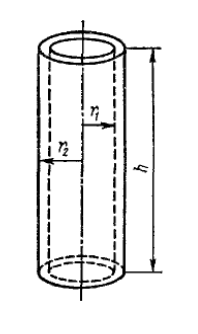
\includegraphics{graphics/t15.PNG}
\end{center}

В таком случае электроёмкость такого конденсатора вычисляется по формуле: $C = \frac{2 \pi \epsilon \epsilon_0 h}{ln(\frac{r_2}{r_1})}$

\section{Расчет электроемкости сферического конденсатора.}

Сферический конденсатор состоит из двух концентрических металлических обкладок сферической формы, радиусы которых соответственно равны $R_1$ и $R_2$.

\begin{center}
    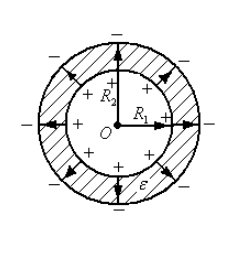
\includegraphics{graphics/t16.PNG}
\end{center}

В таком случае электроёмкость такого конденсатора вычисляется по формуле: $C = \frac{4 \pi \epsilon \epsilon_0 R_1 R_2}{R_2 - R_1}$

\section{Расчет электроемкости двухпроводной линии.}

Двухпроводная линия состоит из двух параллельных цилиндрических провода с радиусами a и расстоянием между осями d.

\begin{center}
    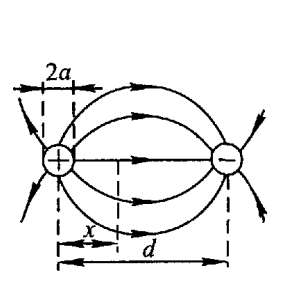
\includegraphics{graphics/t17.PNG}
\end{center}

В таком случае электроёмкость такого конденсатора вычисляется по формуле: $C = \frac{\pi \epsilon \epsilon_0 h}{ln(\frac{d - a}{a})}$

\section{Энергия электрического поля в объеме цилиндрического конденсатора.}

Цилиндрический конденсатор состоит из двух полых коаксиальных металлических цилиндров с радиусами $r_1$ и $r_2$, вставленных один в другой.

\begin{center}
    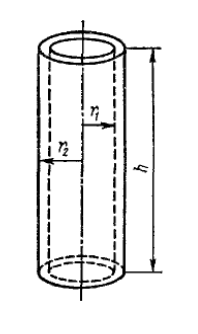
\includegraphics{graphics/t15.PNG}
\end{center}

В таком случае энергия электрического поля равна: $W = \frac{q^2}{2C} = \frac{C U^2}{2} = \frac{qU}{2}$

(Выбираем в зависимости от данных)

А электроёмкость считается по формуле: $C = \frac{2 \pi \epsilon \epsilon_0 h}{ln(\frac{r_2}{r_1})}$

Тогда формулы выходят следующие: $W = \frac{ln(\frac{r_2}{r_1}) q^2}{4 \pi \epsilon \epsilon_0 h} = \frac{\pi \epsilon \epsilon_0 h U^2}{ln(\frac{r_2}{r_1})}$

\section{Энергия электрического поля в объеме сферического конденсатора.}

Сферический конденсатор состоит из двух концентрических металлических обкладок сферической формы, радиусы которых соответственно равны $R_1$ и $R_2$.

\begin{center}
    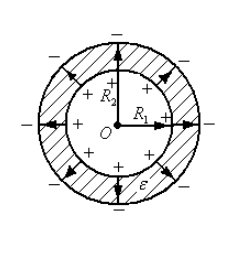
\includegraphics{graphics/t16.PNG}
\end{center}

В таком случае энергия электрического поля равна: $W = \frac{q^2}{2C} = \frac{C U^2}{2} = \frac{qU}{2}$

(Выбираем в зависимости от данных)

А электроёмкость считается по формуле: $C = \frac{4 \pi \epsilon \epsilon_0 R_1 R_2}{R_2 - R_1}$

Тогда формулы выходят следующие: $W = \frac{(R_2 - R_1) q^2}{8 \pi \epsilon \epsilon_0 R_1 R_2} = \frac{2 \pi \epsilon \epsilon_0 R_1 R_2 U^2}{R_2 - R_1}$
\end{document}